% 2018 May 22 - From Jackson+ (2013) study of HAT-P-7 - "Welsh et al. (2010) discovered ellipsoidal variations in the Kepler Q1 data, with an amplitude of 37.3 ppm. They also estimated that the planet’s phase curve has an amplitude of 31.9 ppm..." - So EVs and planet's phase curve has comparable amplitudes.

\documentclass[manuscript]{aastex62}

%% preprint2 produces a double-column, single-spaced document:

%% \documentclass[preprint2]{aastex}

%% Sometimes a paper's abstract is too long to fit on the
%% title page in preprint2 mode. When that is the case,
%% use the longabstract style option.

%% \documentclass[preprint2,longabstract]{aastex}

%% If you want to create your own macros, you can do so
%% using \newcommand. Your macros should appear before
%% the \begin{document} command.
%%
%% If you are submitting to a journal that translates manuscripts
%% into SGML, you need to follow certain guidelines when preparing
%% your macros. See the AASTeX v5.x Author Guide
%% for information.

\newcommand{\kepler}{{\it Kepler}}
\newcommand{\tess}{{\it TESS}}
% \newcommand{\myemail}{skywalker@galaxy.far.far.away}

%% You can insert a short comment on the title page using the command below.

%\slugcomment{Submitted to ApJ, Fall 2018}

%% If you wish, you may supply running head information, although
%% this information may be modified by the editorial offices.
%% The left head contains a list of authors,
%% usually a maximum of three (otherwise use et al.).  The right
%% head is a modified title of up to roughly 44 characters.
%% Running heads will not print in the manuscript style.

\shorttitle{Variability of Kepler-76 b}
\shortauthors{Jackson, Adams, Sandidge, Kreyche, \& Briggs}

%% This is the end of the preamble.  Indicate the beginning of the
%% paper itself with \begin{document}.
\usepackage{hyperref}
\usepackage{graphics,graphicx}

\begin{document}

%% LaTeX will automatically break titles if they run longer than
%% one line. However, you may use \\ to force a line break if
%% you desire.

\title{Variability in the Atmosphere of the Hot Jupiter Kepler-76 b}

%% Use \author, \affil, and the \and command to format
%% author and affiliation information.
%% Note that \email has replaced the old \authoremail command
%% from AASTeX v4.0. You can use \email to mark an email address
%% anywhere in the paper, not just in the front matter.
%% As in the title, use \\ to force line breaks.

\author{Brian Jackson}
\affiliation{Department of Physics, Boise State University, 1910 University Drive, Boise ID 83725-1570 USA}

\author{Elisabeth Adams}
\affiliation{Planetary Science Institute, 1700 E. Ft. Lowell, Suite 106, Tucson, AZ 85719, USA}

\author{Wesley Sandidge}
\affiliation{Department of Physics, Boise State University, 1910 University Drive, Boise ID 83725-1570 USA}

\author{Steven Kreyche}
\affiliation{Department of Physics, Boise State University, 1910 University Drive, Boise ID 83725-1570 USA}
\affiliation{Department of Physics, University of Idaho, Moscow, Idaho 83844-0903, USA}

\author{Jennifer Briggs}
\affiliation{Department of Physics, Boise State University, 1910 University Drive, Boise ID 83725-1570 USA}


%% Notice that each of these authors has alternate affiliations, which
%% are identified by the \altaffilmark after each name.  Specify alternate
%% affiliation information with \altaffiltext, with one command per each
%% affiliation.

%\altaffiltext{1}{bjackson@boisestate.edu}

%% Mark off your abstract in the ``abstract'' environment. In the manuscript
%% style, abstract will output a Received/Accepted line after the
%% title and affiliation information. No date will appear since the author
%% does not have this information. The dates will be filled in by the
%% editorial office after submission.

\begin{abstract}

\end{abstract}

%% Keywords should appear after the \end{abstract} command. The uncommented
%% example has been keyed in ApJ style. See the instructions to authors
%% for the journal to which you are submitting your paper to determine
%% what keyword punctuation is appropriate.

\keywords{}

%% From the front matter, we move on to the body of the paper.
%% In the first two sections, notice the use of the natbib \citep
%% and \citet commands to identify citations.  The citations are
%% tied to the reference list via symbolic KEYs. The KEY corresponds
%% to the KEY in the \bibitem in the reference list below. We have
%% chosen the first three characters of the first author's name plus
%% the last two numeral of the year of publication as our KEY for
%% each reference.


%% Authors who wish to have the most important objects in their paper
%% linked in the electronic edition to a data center may do so by tagging
%% their objects with \objectname{} or \object{}.  Each macro takes the
%% object name as its required argument. The optional, square-bracket 
%% argument should be used in cases where the data center identification
%% differs from what is to be printed in the paper.  The text appearing 
%% in curly braces is what will appear in print in the published paper. 
%% If the object name is recognized by the data centers, it will be linked
%% in the electronic edition to the object data available at the data centers  
%%
%% Note that for sources with brackets in their names, e.g. [WEG2004] 14h-090,
%% the brackets must be escaped with backslashes when used in the first
%% square-bracket argument, for instance, \object[\[WEG2004\] 14h-090]{90}).
%%  Otherwise, LaTeX will issue an error. 


\section{Introduction}

\section{Data Analysis}
\subsection{Data Conditioning}
For each system's light curve, we applied the following steps to condition each quarter's long-cadence (i.e., 30-min integration times) data:
\begin{enumerate}
\item We subtracted the median value from each quarter's PDCSAP\_FLUX time-series before dividing through by that same median value.
\item We next applied a median boxcar filter with a window size equal to four orbital periods. We had experimented with window sizes from one up to 15 orbital periods (holding fixed the transit parameters to those reported in \citealt{2013ApJ...771...26F}), fitting the out-of-transit photometric signals described below using the Levenberg-Marquardt algorithm (LM) \citep{newville_2014_11813}, including the planet's eclipse and phase curve; four orbital periods maximized the eclipse depth and minimized the distortion to the phase curve using all available data. To mitigate edge-effect distortions from our boxcar filter, we extended the time-series out a full window length beyond both ends by reflecting the original time-series across its boundary.
\item Finally, we stitched each quarter's conditioned data into one long time-series and subtracted the average value of the planet's eclipse (i.e., we zeroed out the eclipse) because, in principle, only the star's light registers during that phase, setting the baseline against which to measure the photometric variations. Since our phase curve model allows for an arbitrary offset value, zeroing out the eclipse had no physical significance.
\end{enumerate}
Figure \ref{fig:raw-conditioned-data_Analysis_of_Kepler76b} illustrates a portion of the raw and conditioned time-series for Kepler-76 b. 

\subsection{Analysis and Results}
\subsubsection{Analyzing All Data Folded Together}
After applying the above conditioning procedure, we fit a series of photometric models to all the available data. We first analyzed the out-of-transit portion of Kepler-76 b's light curve since those signals (the ellipsoidal variations, the planet's phase curve, and the Doppler beaming signal) are independent of the transit and can, in principle, contribute to the transit portion (although in practice, their effects are negligible). 

We folded all data on the best-fit period reported by \citet{2013ApJ...771...26F} and masked out the transit and eclipse portions of the light curve to which we fit the following model:
\begin{equation}
    % \Delta F & = & F_0 - A_{\rm ellip} \cos \left(2\times2\pi\phi \right) + A_{\rm beam} \sin \left(2 \pi\phi \right) - A_{\rm planet} \cos \big(2\pi \left( \phi - \delta \right)\big)\nonumber \\
    \Delta F & = & F_0 - A_{\rm ellip} \cos \left(2\times2\pi\phi \right) + A_{\rm sin} \sin \left(2 \pi\phi \right) - A_{\rm cos} \cos \left(2\pi \phi \right),
\label{eqn:BEER_curve}
\end{equation}
where $F_0$ represents a constant baseline, $\phi$ the orbital phase ($\phi = 0$ at mid-transit), and the second term the ellipsoidal variations induced by the planet's tidal gravity \citep{2010ApJ...713L.145W} with $A_{\rm ellip}$ its amplitude. The third and fourth terms represent a combination of the Doppler beaming signal \citep{2003ApJ...588L.117L} and the planet's reflected/thermally emitted phase curve, with allowance for an offset in the curve's maximum from superior conjunction at $\phi = 0.5$ \citep{2013ApJ...771...26F}. We also allowed the per-point uncertainty (``noise'') to be a free parameter and estimated the model likelihood $L$ as
\begin{equation}
    \ln L = -\frac{1}{2} \sum_i \bigg( \dfrac{ d(t_{\rm i}) - m(t_{\rm i}) }{\sigma} \bigg)^2 + \ln \left( 2 \pi \sigma^2 \right),
    \label{eqn:likelihood}
\end{equation}
where $d(t_{\rm i})$ is the datum at time $t_{\rm i}$, $m(t_{\rm i})$ the model for that same time, and $\sigma$ the per-period uncertainty. With this likelihood, we used a Markov-Chain Monte-Carlo (MCMC) analysis \citep{2013PASP..125..306F} with 100 walker chains, each with 5,000 links and a burn-in phase of 2,500 links. We aimed for convergence by requiring small auto-correlation times \citep[e.g][]{geyer1992} for the mean chain of each fit parameter (none exceeded 80 links) and all Geweke Z-scores \citep{Geweke92evaluatingthe} of about 3 or less. 

Traditionally, the beaming and planetary phase curve signals are treated separately through the combination $A_{\rm beam} \sin \left(2 \pi\phi \right) - A_{\rm planet} \cos \big(2\pi \left( \phi - \delta \right)\big)$. This expression can be re-cast using $A_{\rm sin} = A_{\rm beam} - A_{\rm planet} \sin \left( 2 \pi \delta \right)$ and $A_{\rm cos} = A_{\rm planet} \cos \left( 2 \pi \delta \right)$. Since the beaming and planetary phase curve signals have the same frequency (once per orbit), and the phase offset $\delta$ allows them to phase up (at least in principle), they are degenerate; independent fits for $A_{\rm beam}$, $A_{\rm planet}$, and $\delta$ are not possible.

Figure \ref{fig:BEER-curve-fit_Analysis_of_Kepler76b} shows the fit and residuals for Equation \ref{eqn:BEER_curve} to the data set. Figure \ref{fig:BEER-curve-fit-params_Analysis-of-Kepler76b} shows the resulting best-fit parameters, while Figure \ref{fig:Aplanet-delta-fit-params_Analysis-of-Kepler76b} shows the corresponding range of values for $A_{\rm planet}$ and $\delta$. To generate the latter figure, we calculated $A_{\rm beam}$ from the radial-velocity semi-amplitude $K_{\rm z} = 0.306 \pm 0.020$ km/s reported in \citet{2013ApJ...771...26F} using $A_{\rm beam} = 4\ \alpha_{\rm beam}\ K_{\rm z}/c = 3.8 \pm 0.3$ ppm, where $c$ the speed of light \citep{2003ApJ...588L.117L} -- we did not use the $A_{\rm beam}$-value reported in \citet{2013ApJ...771...26F}. Then, we Monte-Carlo-sampled 250,000 times from a Gaussian distribution for $A_{\rm beam}$ (with the mean and width given above), as well as the MCMC chains for $A_{\rm sin}$ and $A_{\rm cos}$. Figure \ref{fig:Aplanet-delta-fit-params_Analysis-of-Kepler76b} shows the clear correlation between $A_{\rm beam}$ and $\delta$. As a final check, we fit the out-of-transit/out-of-eclipse data with an LM approach, holding $A_{\rm beam}$ fixed at 13.5 ppm, as reported in \citet{2013ApJ...771...26F}, and were able to recover the reported $A_{\rm planet}$ but not the $\delta$-value.
%previously, in line 130, "We next ..." was used, so to be a smidge different, line 163 can start with "We then ...".  We don't want first two sentences of this paragraph to be "Word, we" as it currently is/was "Next, we" and "Importantly, we".

We then analyzed the in-transit portion of the light curve. Importantly, we accounted for \kepler's finite integration time of 30-min-per-point by super-sampling each point (the finite integration had no significant effect on the Equation \ref{eqn:BEER_curve} model). By first subtracting the Equation \ref{eqn:BEER_curve} model from the in-transit portion of the light curve, we removed its (very small) influence on the transit. Then, we used LM to fit a standard transit curve with quadratic limb-darkening \citep{2002ApJ...580L.171M}\footnote{As implemented in PyAstronomy -- \url{https://github.com/sczesla/PyAstronomy}.} to that portion of the time-series within two transit durations of the reported mid-transit time, allowing the out-of-transit baseline to vary. This analysis netted initial best-fit transit parameters: $a/R_\star$, the ratio of the planet's semi-major axis to the stellar radius; $b$, the impact parameter; and $R_{\rm p}/R_\star$, the planet-to-star radius ratio. We assumed the orbital eccentricity is equal to zero based on the photometric and radial velocity analyses in \citet{2013ApJ...771...26F} and held fixed the limb-darkening coefficients $\gamma_1 = 0.313$ and $\gamma_2 = 0.304$. We explored two other sets of quadratic limb-darkening coefficients, estimated assuming the stellar parameters from \citet{2013ApJ...771...26F} and using the model from \citet{2015MNRAS.450.1879E}, but found different values had negligible impact on our transit analysis. 
%in the paragraph above, you state that "this analysis netted initial best-fit parameters" which is fine and all, but . . . you then describe three variables a/R* and b and Rp/R*. These variables have not been introduced in a previous equation, nor in the paragraph.  However, IF these variable are in fact THE "best-fit transit parameters" then the sentence(s) would benefit (hopefully) from the changes I made.

To check for transit-timing variations, we fit each individual transit (with the full orbital light curve this time and not just the in-transit portion) using LM again and held fixed all transit parameters except the mid-transit times and out-of-transit baseline. For uncertainties, we took the square root of the diagonal elements of the resulting covariance matrix \citep[p.~790]{Press:2007:NRE:1403886} and confirmed the accuracy of the mid-transit times and uncertainties by also fitting transit curves with a Markov-Chain Monte-Carlo (MCMC) analysis \citep{2013PASP..125..306F} to several individual transits -- we achieved convergence with 100 walkers, each a chain of 1,000 links and a burn-in phase of 300 links. Although most single transits are detectable, they usually comprise one or two data points and so provide no useful constraints on parameters other than the mid-transit times. Finally, we fit the collection of mid-transit times with linear and quadratic ephmerides using an MCMC analysis (100 walker chains, 5,000 links in each with a burn-in of 1,500 links) and found no significant departure from the latter. We also found no significant periodicities using a Lomb-Scargle periodogram \citep{1976Ap&SS..39..447L, 1982ApJ...263..835S}. Figure \ref{fig:TTVs_Analysis_of_Kepler76b} shows the resulting transit ephemeris, which is completely consistent with that reported in \citet{2013ApJ...771...26F}. 

With this updated ephemeris, we folded together all available data and fit the resulting transit portion of the light curve, with free parameters $a/R_\star$, $b$, $R_{\rm p}/R_\star$, and an estimate of the per-point noise (again using Equation \ref{eqn:likelihood} for the likelihood). We used the same MCMC analysis as above, with 100 walker chains, each with 32,000 links and a burn-in phase of 16,000 links. We aimed for convergence by requiring small auto-correlation times \citep[e.g][]{geyer1992} for the mean chain of each fit parameter (none exceeded 250 links) and all Geweke Z-scores \citep{Geweke92evaluatingthe} of about 3 or less. Figure \ref{fig:folded-transit-corner-plot_Analysis-of-Kepler76b} shows the resulting parameter distributions, with the best-fit values and uncertainties given in Table X, and Figure \ref{fig:final_best_fit_transit_Analysis_of_Kepler76b} shows the resulting transit curve and residuals.

\subsubsection{Searching for Eclipse and Planetary Phase Curve Variability}
\label{sec:Searching}
We turned to a search for orbit-to-orbit variability in the planet's phase curve and secondary eclipse. First, we folded together all 944 orbits-worth of data on our best-fit ephemeris and used the LM algorithm to fit the out-of-transit and eclipse portions (accounting for \kepler's finite integration time) to establish the average fit-values -- the result eclipse depth $D = 87 \pm 6$ ppm, a 14.5-$\sigma$ detection. In our search for variability, ideally we'd like to analyze the data for each orbit individually to maximize our time resolution. However, with a 14.5-$\sigma$ detection over 944 orbits for Gaussian noise, we expect that a 3-$\sigma$ detection of the eclipse requires folding together data from about 40 ($=\left( \frac{3}{14.5} \right)^2 \times 944 $) orbits, giving a time resolution of about 60 days. We expect estimates of the parameters $A_{\rm sin}$ and $A_{\rm cos}$ to be more robust, however, since those signals are present throughout most of the orbit (the eclipse only occupies two or three points each orbit). 

For this analysis, we marched a window spanning 10, 20, or 40 orbits from the beginning to the end of the dataset, moving one orbital period at a time. We folded all the out-of-transit points in the window together and fit Equation \ref{eqn:BEER_curve} and an eclipse represented by the same transit light curve model as above but with a variable depth $D$ and limb-darkening parameters set to zero (i.e., a uniform disk). We used the LM algorithm and took the square root of the diagonal of the covariance matrix as the parameter uncertainties (scaled by the square root of the resulting reduced $\chi^2$) -- we compared these uncertainties to those derived from an MCMC analysis for several stacked orbits and found good agreement (to within 1 ppm). 

To avoid having our window span large gaps in the data, we required that a window included a large enough number of data points that at least half the desired number of orbits were represented. For example, for the window spanning 10 orbits, we required at least 5 orbital periods worth of data (i.e., about $360 = 5 \times 1.5\ {\rm days}/30\ {\rm min}$ points). We took the mid-eclipse time to be the mid-transit time plus half an orbital period, again assuming zero orbital eccentricity. Figure \ref{fig:planet-phase-curve-var_Analysis_of_Kepler76b} shows the resulting collection of best-fit parameters for the different windows, where the x-coordinate of each point represents the median observational time for all the points in the window. Since the windows span several orbits and the points are only spaced by one orbital period, the parameter fits are not all statistically independent.

The plots seem to show considerable variability, but comparing the variations to the best-fit average values (top right panel of Figure \ref{fig:planet-phase-curve-var_Analysis_of_Kepler76b}) show that the eclipse depth departs from its average value, 87 ppm, by less than 3-$\sigma$, where $\sigma$ is calculated by adding uncertainties in quadrature \citep[p.~58]{1997ieas.book.....T}. By contrast, $A_{\rm sin}$ and $A_{\rm cos}$ frequently depart by more than 3- and sometimes 5-$\sigma$ from their average values. As expected, though, the more orbits stacked together, the more the variations are averaged out, but even the points involving 40 orbits stacked together (in green) show statistically significant variation. These results, of course, rely on the accuracy of our uncertainty estimates, so we conducted several numerical tests to check them. 

First, we generated and fit several synthetic datasets incorporating Gaussian noise and with the same observational times as the real dataset but holding the phase curve parameters and eclipse depth constant. These fits showed variations visually similar to those in Figure \ref{fig:planet-phase-curve-var_Analysis_of_Kepler76b}, but always the variations in fit parameters are within 3-$\sigma$ of the assumed constant values.

We next gathered and phased up about 7,000 datasets involving 10, 20, or 40 orbits worth of out-of-transit data (10 times the number of points in the left panels in Figure \ref{fig:planet-phase-curve-var_Analysis_of_Kepler76b}) but randomly scattered throughout the whole \kepler\ time-series, i.e. orbits that were not necessarily adjacent in time. We expect that parameter fits to these scattered datasets will show only random scatter, with orbit-to-orbit coherent variations averaged out. We used the Kolmogorov-Smirnov (KS) test \citep[p.~730]{Press:2007:NRE:1403886} to compare the distributions of best-fit parameters (scaled by their respective uncertainties) for these scattered data to the same scaled distributions for the unscattered data (right panels in Figure \ref{fig:planet-phase-curve-var_Analysis_of_Kepler76b}). To judge the range of KS scores we should expect, we randomly sub-sampled the distribution of best-fit parameters for the scattered data 10,000 times and compared these subsamples to one another. The KS test comparisons indicated that the distribution of eclipse depths for the unscattered data resembled closely the distribution for the scattered data, indicating that the variations in the top left panel of Figure \ref{fig:planet-phase-curve-var_Analysis_of_Kepler76b} are consistent with statistical noise. The KS test comparisons for $A_{\rm sin}$ suggests the distribution for the unscattered data is unlikely (with a KS probabilities of a few 0.1\%) but within the range expected for noise. By contrast, the KS test comparisons for $A_{\rm cos}$ are inconsistent with noise (KS probabilities $<10^{-11}$ when 40 orbits are stacked together), indicating the variations in Figure \ref{fig:planet-phase-curve-var_Analysis_of_Kepler76b} are not simply due to noise. This trend is not surprising -- we typically detected the $A_{\rm cos}$ signal at greater significance than the $A_{\rm sin}$ and eclipse signals. Moreover, since $\delta$ is expected to be small, $A_{\rm sin} \approx A_{\rm beam}$ which should remain constant.

We also employed the same orbit stacking and phasing and fit transit radii (holding other transit parameters fixed) to look for correlations with $A_{\rm cos}$. If the variations in $A_{\rm cos}$-values arise from some stellar or instrumental effect, we might expect the transit depth to vary in concert with $A_{\rm cos}$; however we found no robust linear correlation.

As a final check, we performed an injection-recovery test for which we generated a synthetic dataset designed to closely mimic the original dataset and include the variations in phase curve parameters shown in Figure \ref{fig:planet-phase-curve-var_Analysis_of_Kepler76b}. For this test, we divided up the full time-series into individual orbits, calculating the mid-transit time for each orbit. We linearly interpolated to that mid-transit time from among the phase curve parameters for 10 orbits stacked together (blue points in Figure \ref{fig:planet-phase-curve-var_Analysis_of_Kepler76b}) to determine the phase curve parameters for the orbit. We generated a phase curve model for that orbit and subtracted it from the original, unconditioned time-series (i.e., from the data shown in the top panel of Figure \ref{fig:raw-conditioned-data_Analysis_of_Kepler76b}). Then, we shifted all the mid-transit times forward in time by about 800 days, i.e., half the maximum observational time in the \kepler\ dataset -- mid-transit times that moved out beyond this maximum time, we wrapped back around to the beginning of the dataset. We then injected synthetic phase curve signals back into the shifted data but this time using the phase curve parameters from the original mid-transit times. This approach has the effect of retaining the time-ordered structure to the phase curve variations while planting the phase curves in a different noise environment. Presumably, if we can recover the phase curve parameters, they are robust against noise. Indeed, after re-conditioning these shifted, synthetic data, we were able to recover the vast majority of parameters to within uncertainties. Not surprisingly, for the points not recovered successfully, most were associated with the eclipse depth, which was detected with the least signal-to-noise originally.

\section{Discussion and Conclusions}
From Figure \ref{fig:planet-phase-curve-var_Analysis_of_Kepler76b}, we can see that $A_{\rm cos}$ conservatively varies by about $\pm 40$\% around the median value of $51 \pm 1$ ppm. Since $\delta$ is small ($-8.6^\circ \pm 1.3^\circ$), at the first order, we can attribute the variations in $A_{\rm cos}$ to variations in $A_{\rm planet}$. As indicated in Section \ref{sec:Searching} above, although $A_{\rm sin}$ seems to vary (Figure \ref{fig:planet-phase-curve-var_Analysis_of_Kepler76b}, those variations appear to be of marginal statistical significance, and so we cannot confidently claim to see variations in $\delta$.

Assuming complete redistribution of insolation, the dayside temperature of Kepler-76 b in radiative equilibrium approaches 2,300 K, which puts a significant fraction of its blackbody curve within the \kepler\ bandpass. XX And so what...? -- era XX

Figure \ref{fig:eclipse_estimates} shows estimates of signal-to-noise ratios (SNR) expected for secondary eclipses observed by \tess\ based on the synthetic population of planets in the \tess\ yield calculations from \citet{2018arXiv180405050B}. For each synthetic planet from that study, we estimated the eclipse depth $\Delta$ for the case that the planet reflects all of the light it receives from the star (shown in blue) and for the case that the planet emits (and absorbs) light as a perfect blackbody (shown in orange). For the former case, the eclipse depth is given as $\frac{1}{4} \left( \frac{R_{\rm p}}{a} \right)^2$, where $R_{\rm p}$ is the planetary radius and $a$ is the orbital semi-major axis. We then estimated the corresponding SNR by multiplying the transit SNRs given for each planet by planet-star radius ratio squared and then by $\Delta_{\rm reflected}$. For the latter case, we used the stellar insolation given for each planet and assumed dayside thermal equilibrium with zero albedo for each planet to estimate a brightness temperature and convolved the resulting blackbody curve against the \tess\ spectral response function\footnote{https://tessgi.github.io/TessGiWebsite/the-tess-space-telescope.html}. We combined the insolation and planet's orbital distance to estimate the stellar effective temperature and, likewise, convolved the corresponding blackbody curve against the response function. Finally, we divided the planet's convolved brightness by the star's and used the re-scaled transit SNR to calculate the SNR for the thermally emitted eclipse. Figure \ref{fig:eclipse_estimates} only shows those SNR-values $> 3$, among which the vast majority (54 of 62 total) have $R_{\rm p} \geq 10\ R_{\rm Earth}$.

The synthetic population from \citet{2018arXiv180405050B} included 4,553 planets, and Figure \ref{fig:eclipse_estimates} suggests only about 1\% of these may have secondary eclipses detectable for \tess. However, among those, our calculation suggests that the eclipse signals will be considerably more sensitive to emitted than reflected light, in contrast to the eclipses observed by \kepler\ (ref), which owes largely to the fact that the \tess\ spectral response function is more sensitive at longer wavelengths than that of \kepler. Presumably, this different sensitivity also means detectable \tess\ eclipses will probe atmospheric thermal structures more than \kepler\ eclipses could.

% XXX and something about eclipse variability XXX

% How detectable will be the ellipsoidal variations?

\acknowledgments 
This study is based on work supported by NASA under Grant no.~NNX15AB78G issued through the Astrophysical Data Analysis Program by the Science Mission Directorate. 

%% To help institutions obtain information on the effectiveness of their
%% telescopes, the AAS Journals has created a group of keywords for telescope
%% facilities. A common set of keywords will make these types of searches
%% significantly easier and more accurate. In addition, they will also be
%% useful in linking papers together which utilize the same telescopes
%% within the framework of the National Virtual Observatory.
%% See the AASTeX Web site at http://aastex.aas.org/
%% for information on obtaining the facility keywords.

%% After the acknowledgments section, use the following syntax and the
%% \facility{} macro to list the keywords of facilities used in the research8
%% for the paper.  Each keyword will be checked against the master list during
%% copy editing.  Individual instruments or configurations can be provided 
%% in parentheses, after the keyword, but they will not be verified.

\facility{Kepler}.
\software{numpy, astropy, statsmodels, scipy, lightkurve, BEER\_curve, PyAstronomy, emcee, get\_lds \citep{2015MNRAS.450.1879E}}

\bibliographystyle{aasjournal}
\bibliography{bibliography}

\begin{figure}
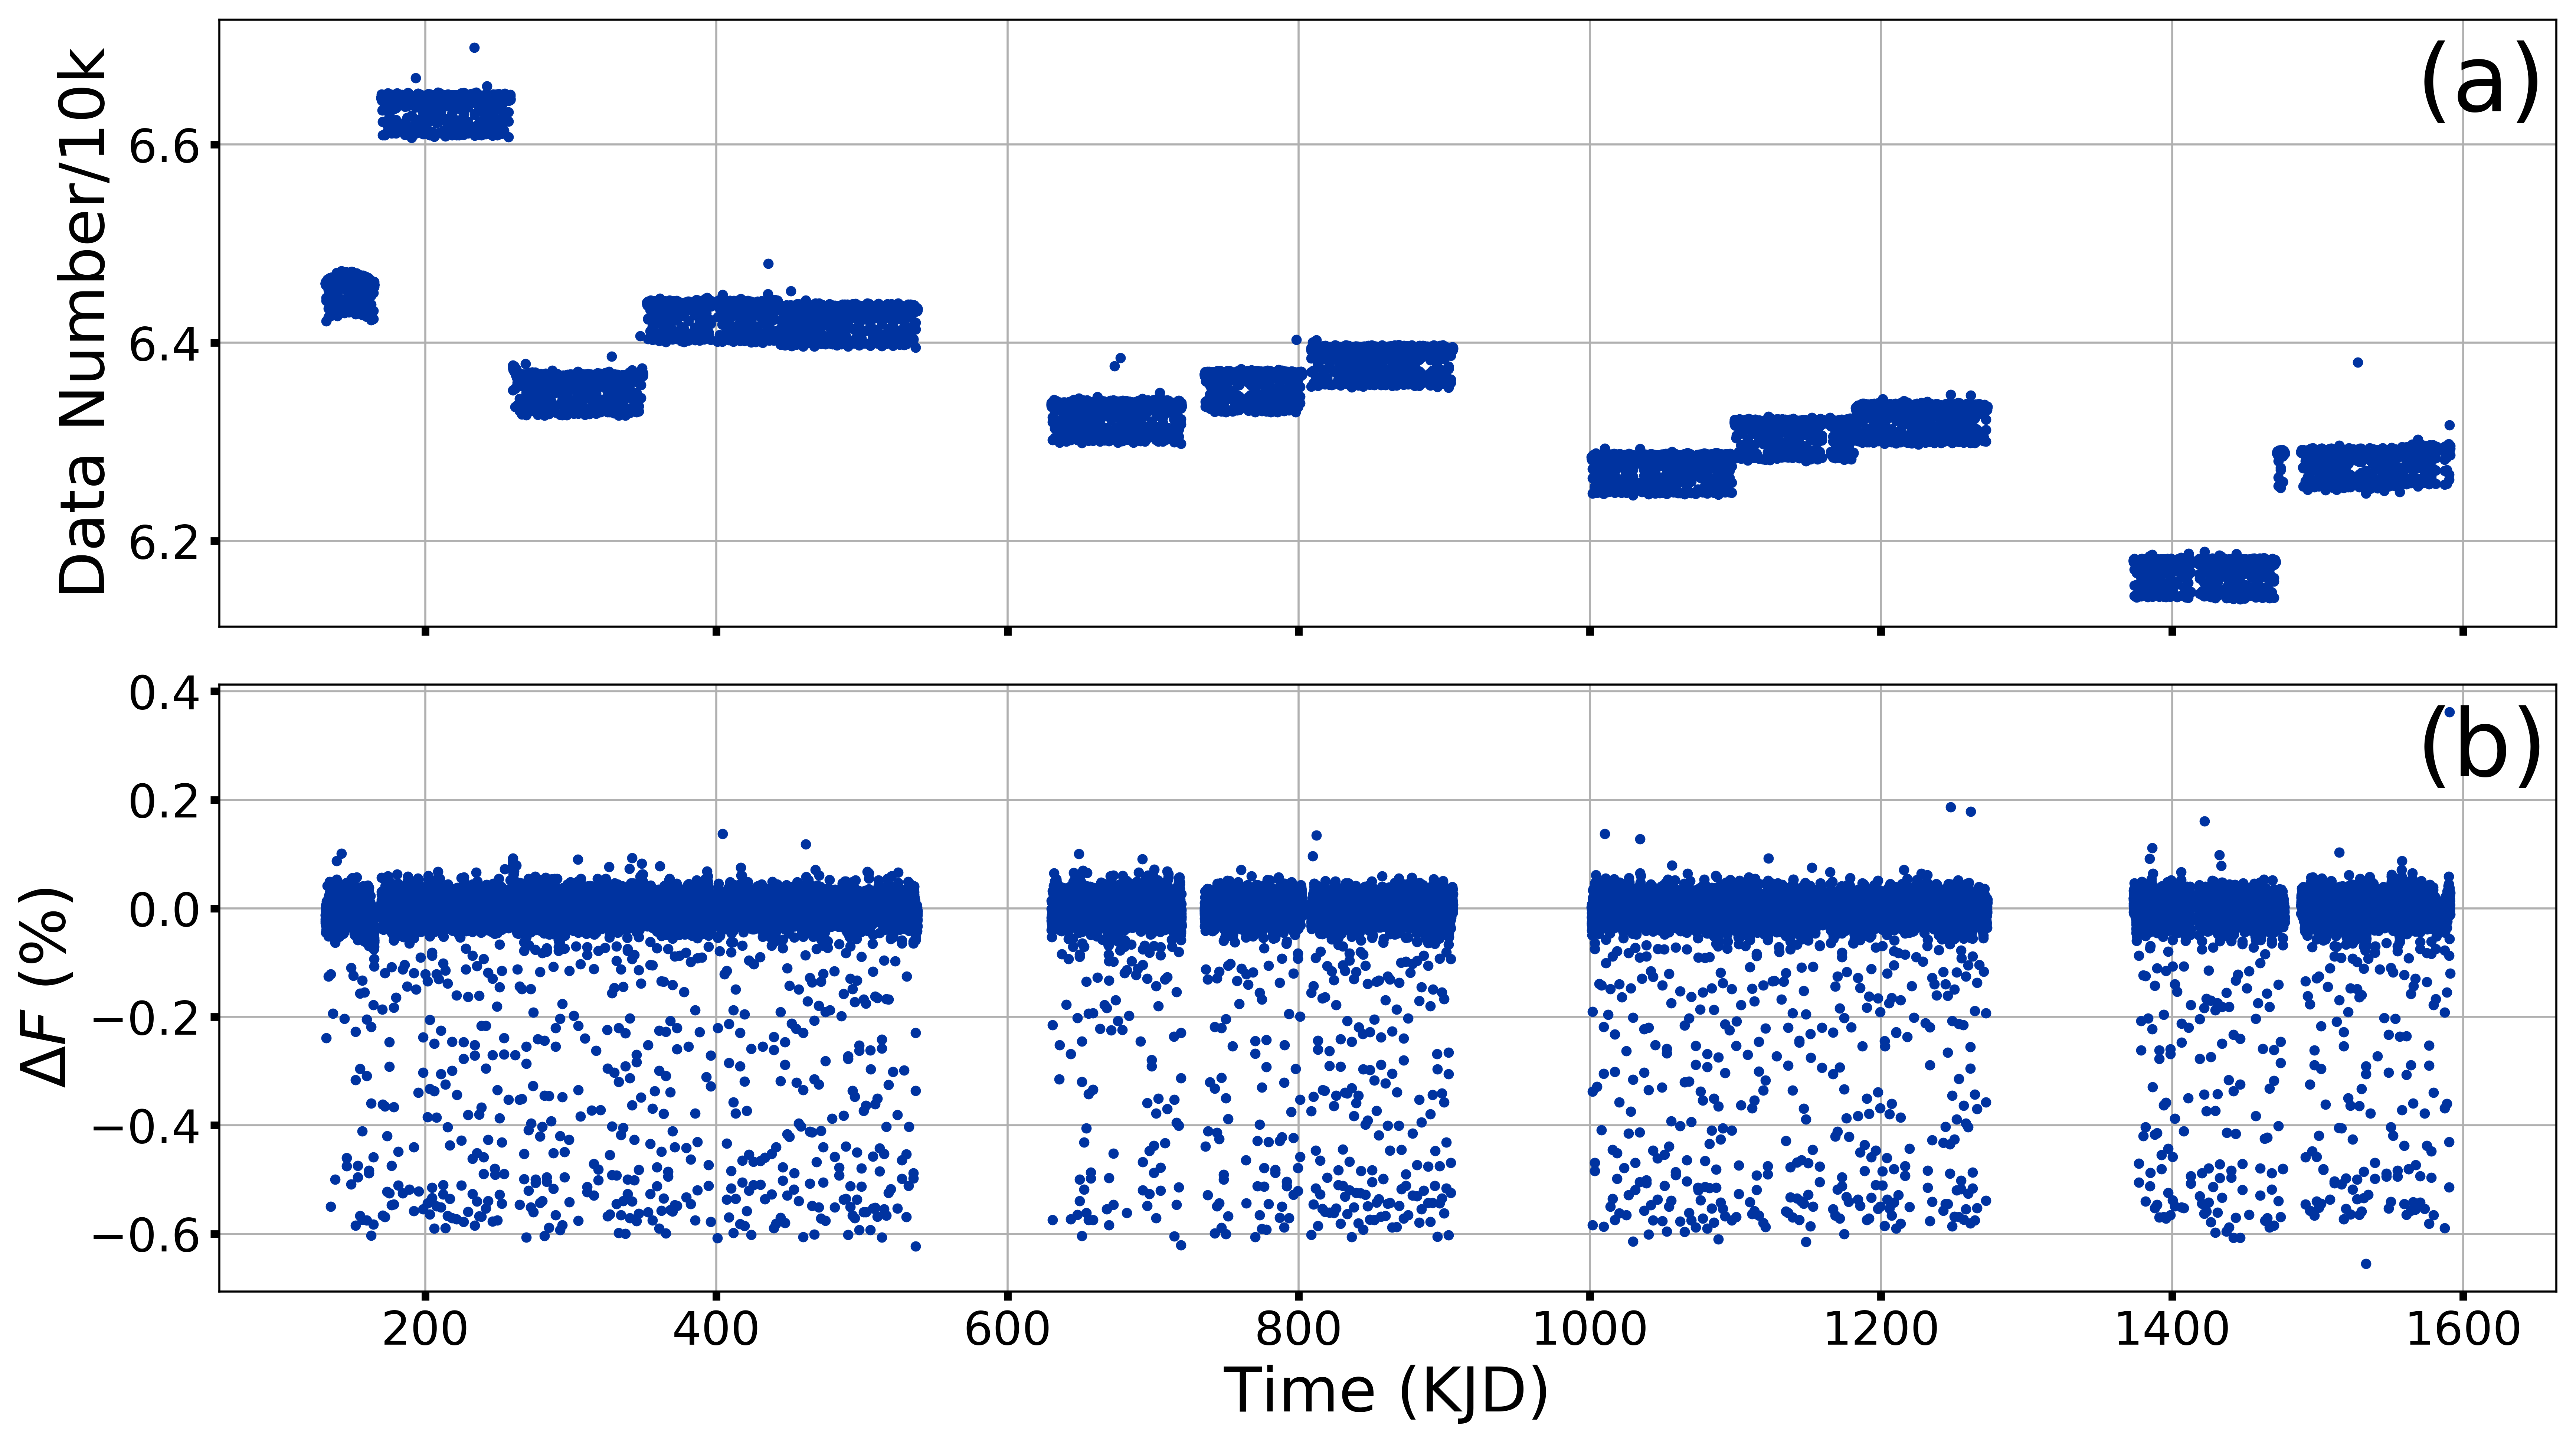
\includegraphics[width=\textwidth]{raw-conditioned-data_Analysis_of_Kepler76b.png}
\caption{The quarter-by-quarter (a) raw and (b) conditioned PDCSAP\_FLUX. Time along the x-axis is shown in the \kepler\ mission's barycentric Julian date minus 2454833 (midnight on 2009 January 1), and the y-axes show variations in flux.\label{fig:raw-conditioned-data_Analysis_of_Kepler76b}}
\end{figure}

\begin{figure}
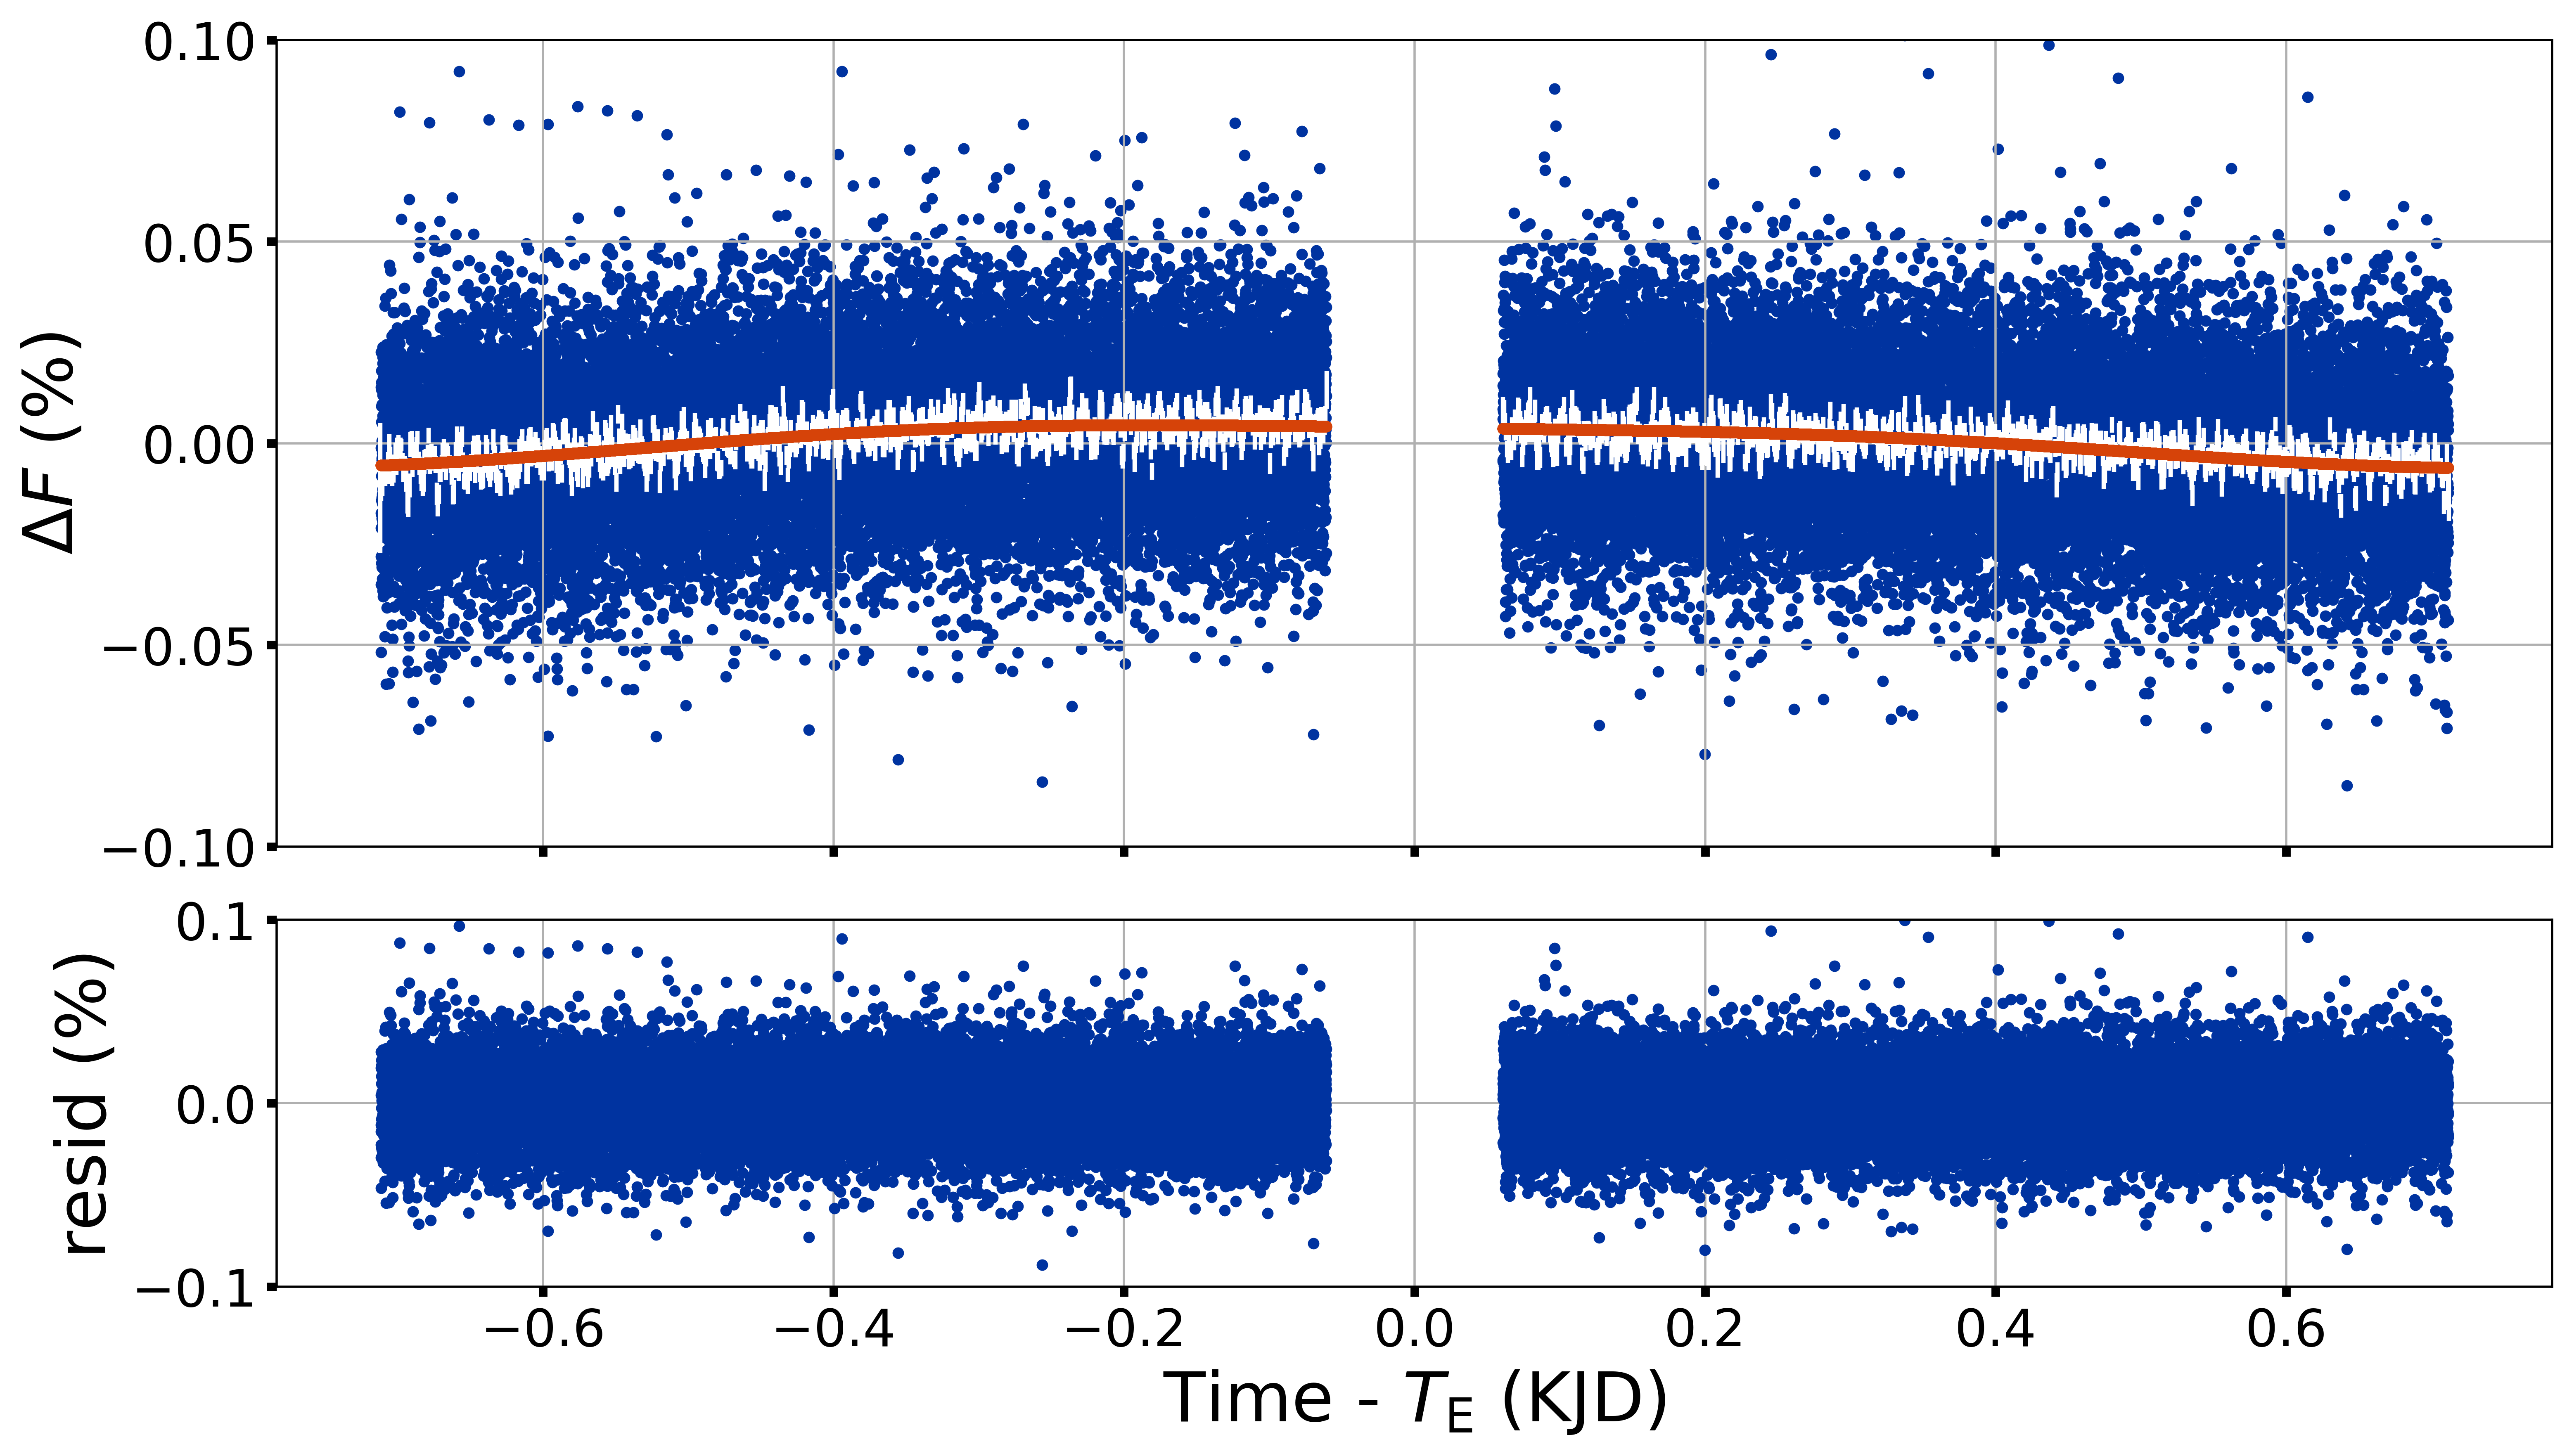
\includegraphics[width=\textwidth]{BEER-curve-fit_Analysis_of_Kepler76b.png}
\caption{The blue points in the top panel show photometric measurements for Kepler-76 outside of eclipse and transit folded on the ephemeris reported in \citet{2013ApJ...771...26F}. The white points show these same data binned in 1-min-wid bins with error bars showing the standard deviation in each bin. The solid orange line shows our best-fit model (Equation \ref{eqn:BEER_curve}), while the dashed black line shows that from \citet{2013ApJ...771...26F}. The bottom panel shows the residuals between our model and the data.\label{fig:BEER-curve-fit_Analysis_of_Kepler76b}}
\end{figure}

\begin{figure}
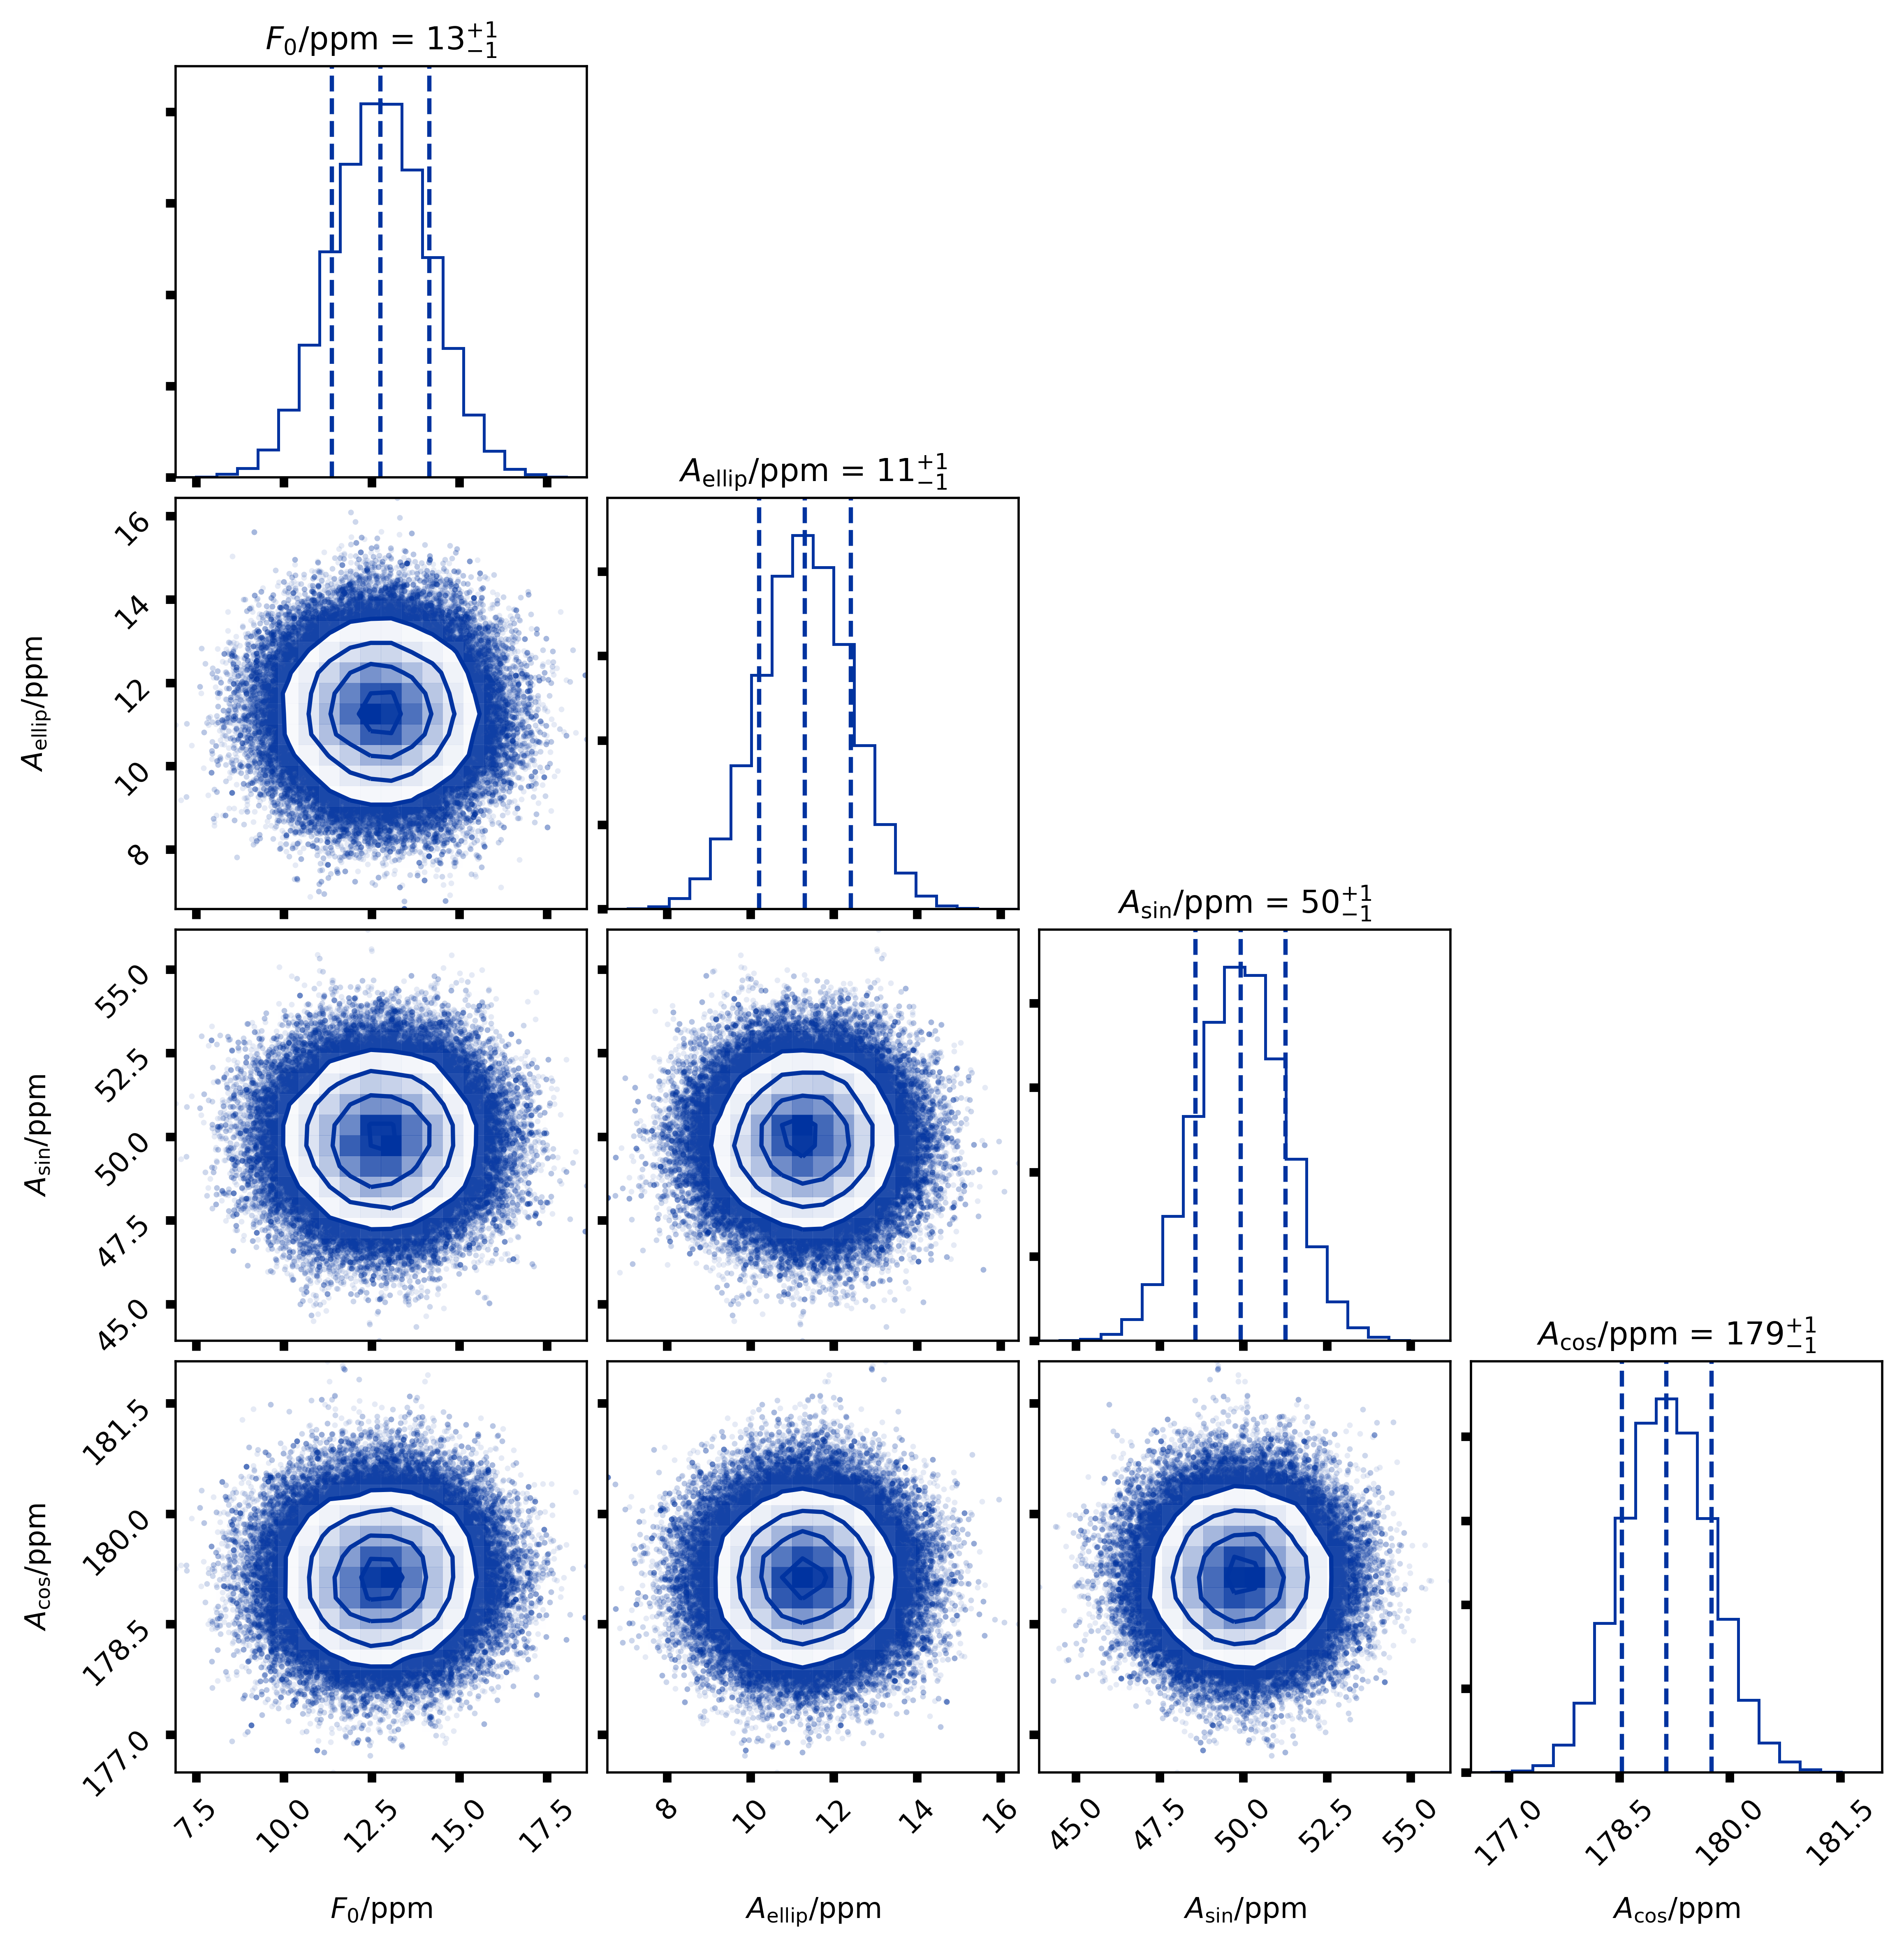
\includegraphics[width=\textwidth]{BEER-curve-fit-params_Analysis-of-Kepler76b.png}
\caption{The posterior distributions for the best-fit parameters for the model described by Equation \ref{eqn:BEER_curve} and corresponding to the orange curve in Figure \ref{fig:BEER-curve-fit_Analysis_of_Kepler76b}. \label{fig:BEER-curve-fit-params_Analysis-of-Kepler76b}}
\end{figure}

\begin{figure}
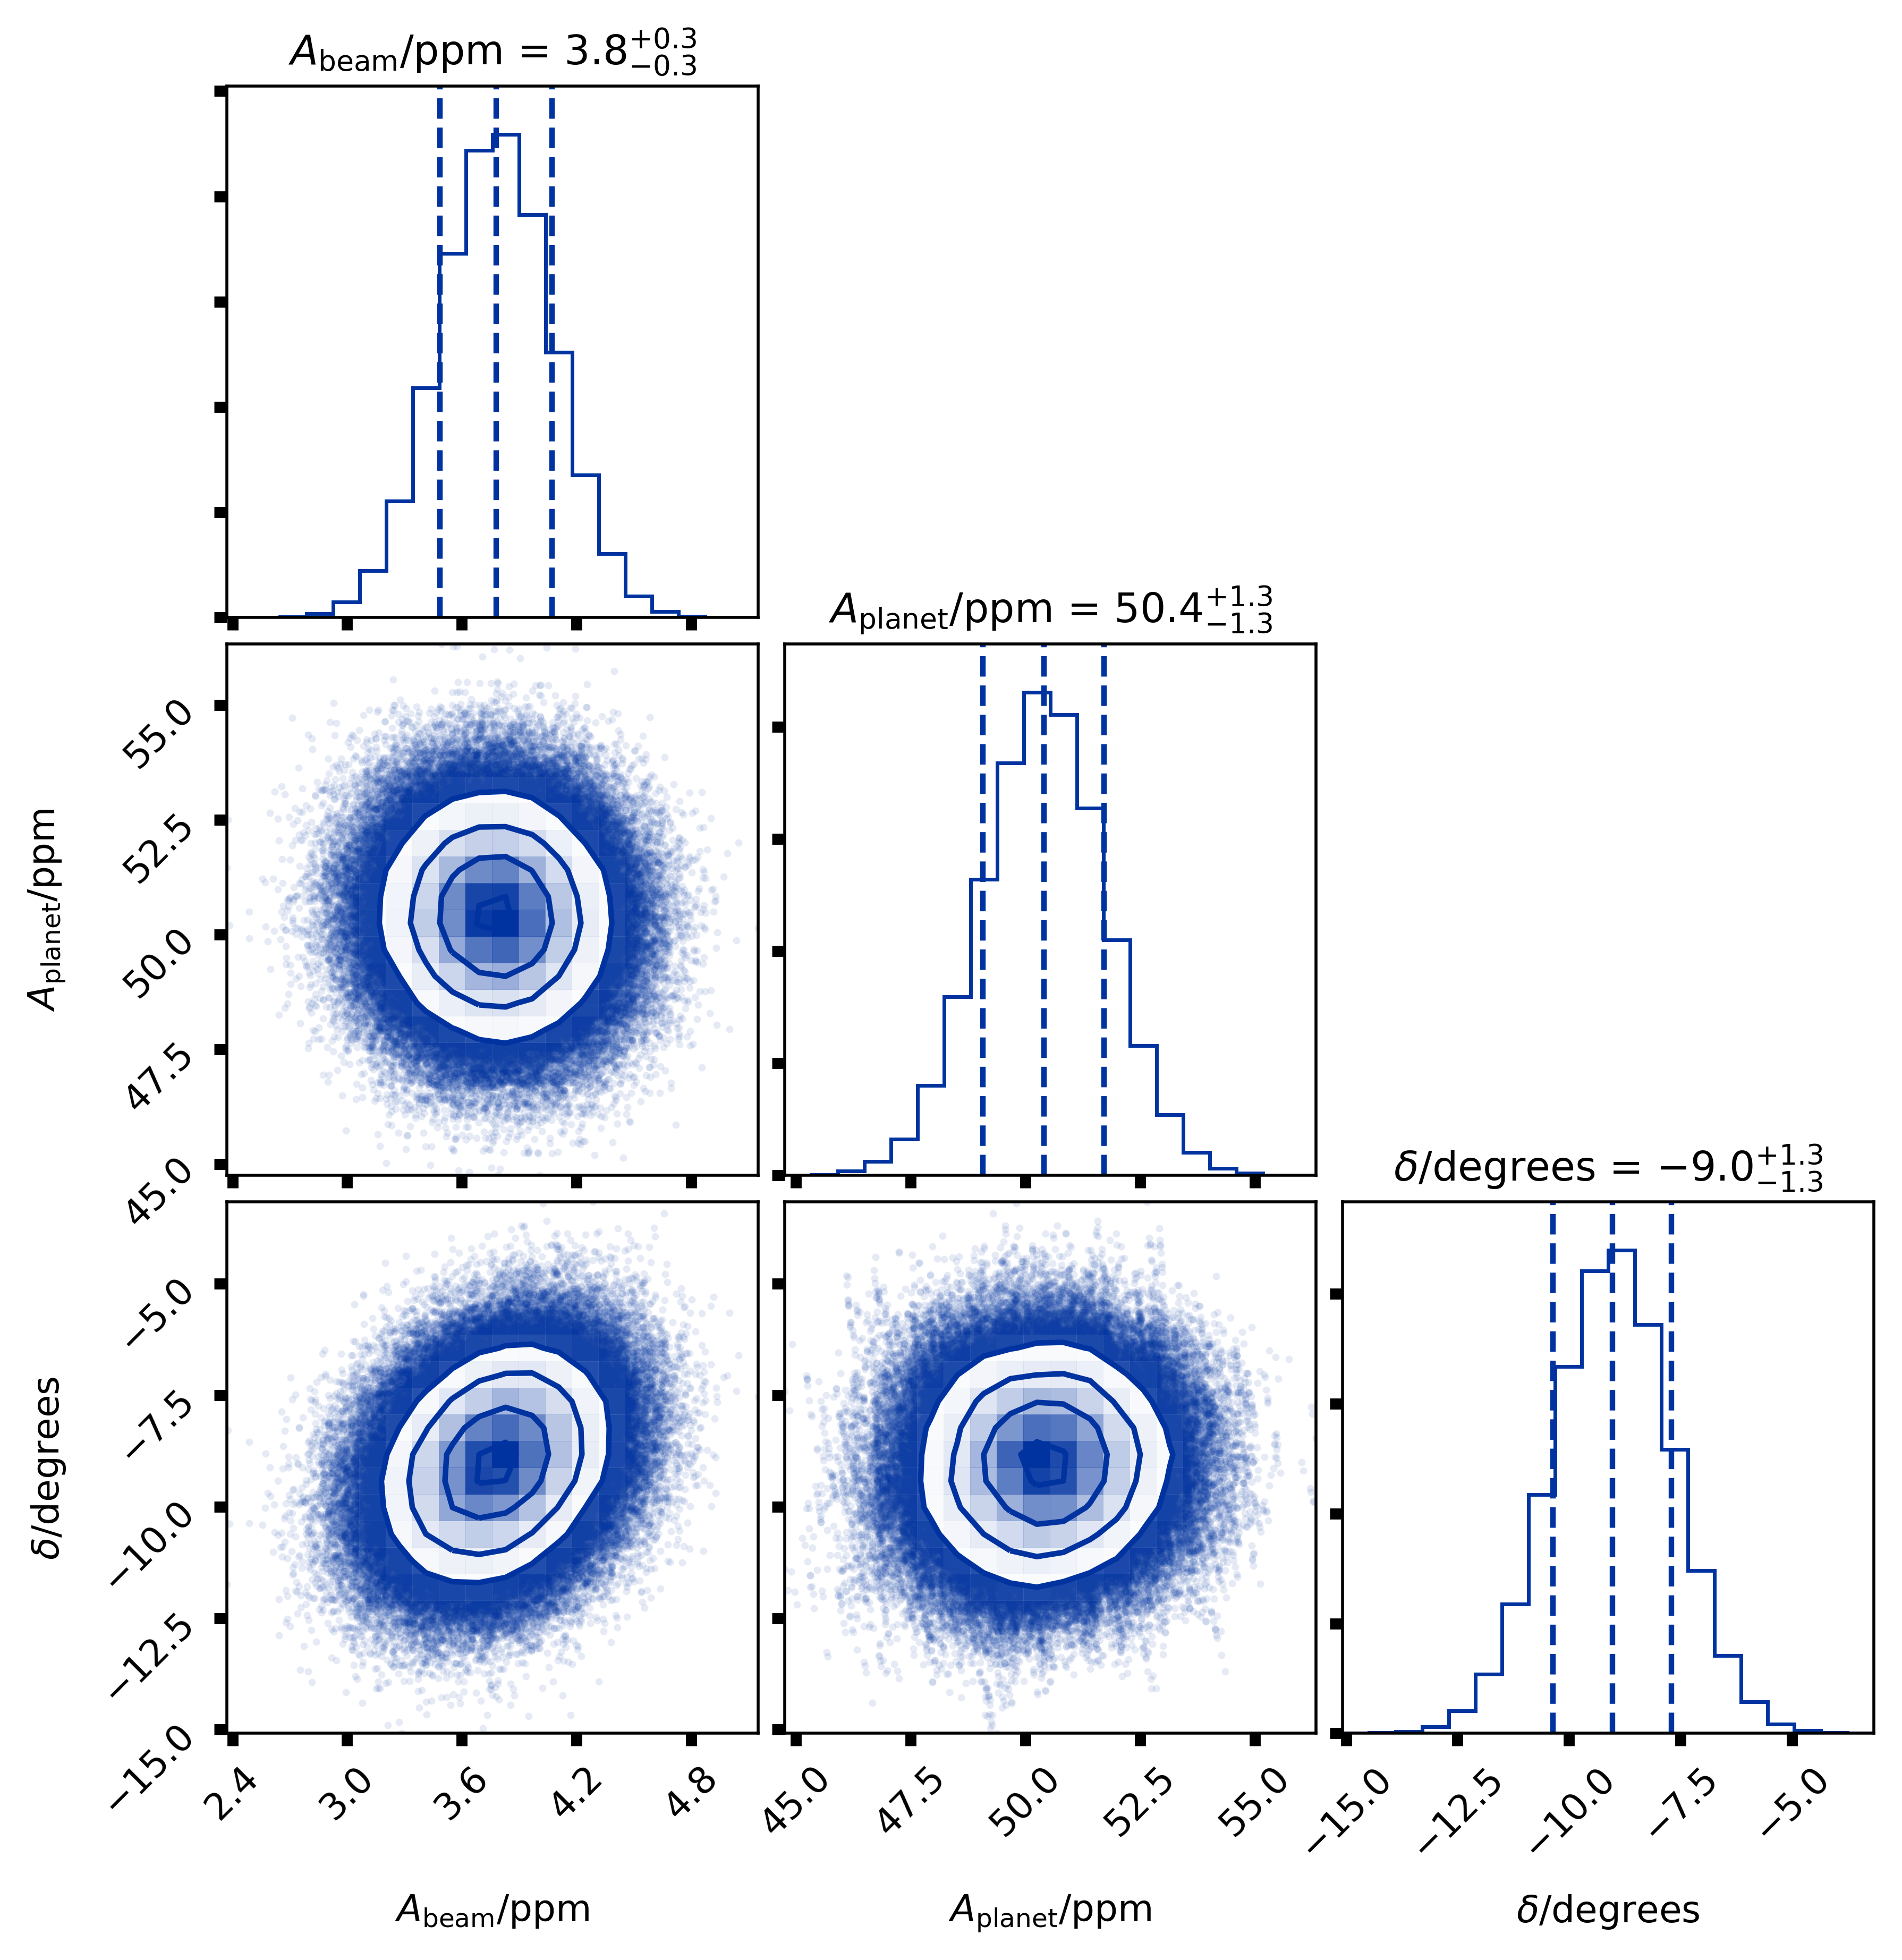
\includegraphics[width=\textwidth]{Aplanet-delta-fit-params_Analysis-of-Kepler76b.png}
\caption{The posterior distributions for the amplitude of the planet's phase curve and its phase offset, assuming the beaming signal amplitude implied by the radial velocity semi-amplitude reported in \citet{2013ApJ...771...26F}. \label{fig:Aplanet-delta-fit-params_Analysis-of-Kepler76b}}
\end{figure}

\begin{figure}
    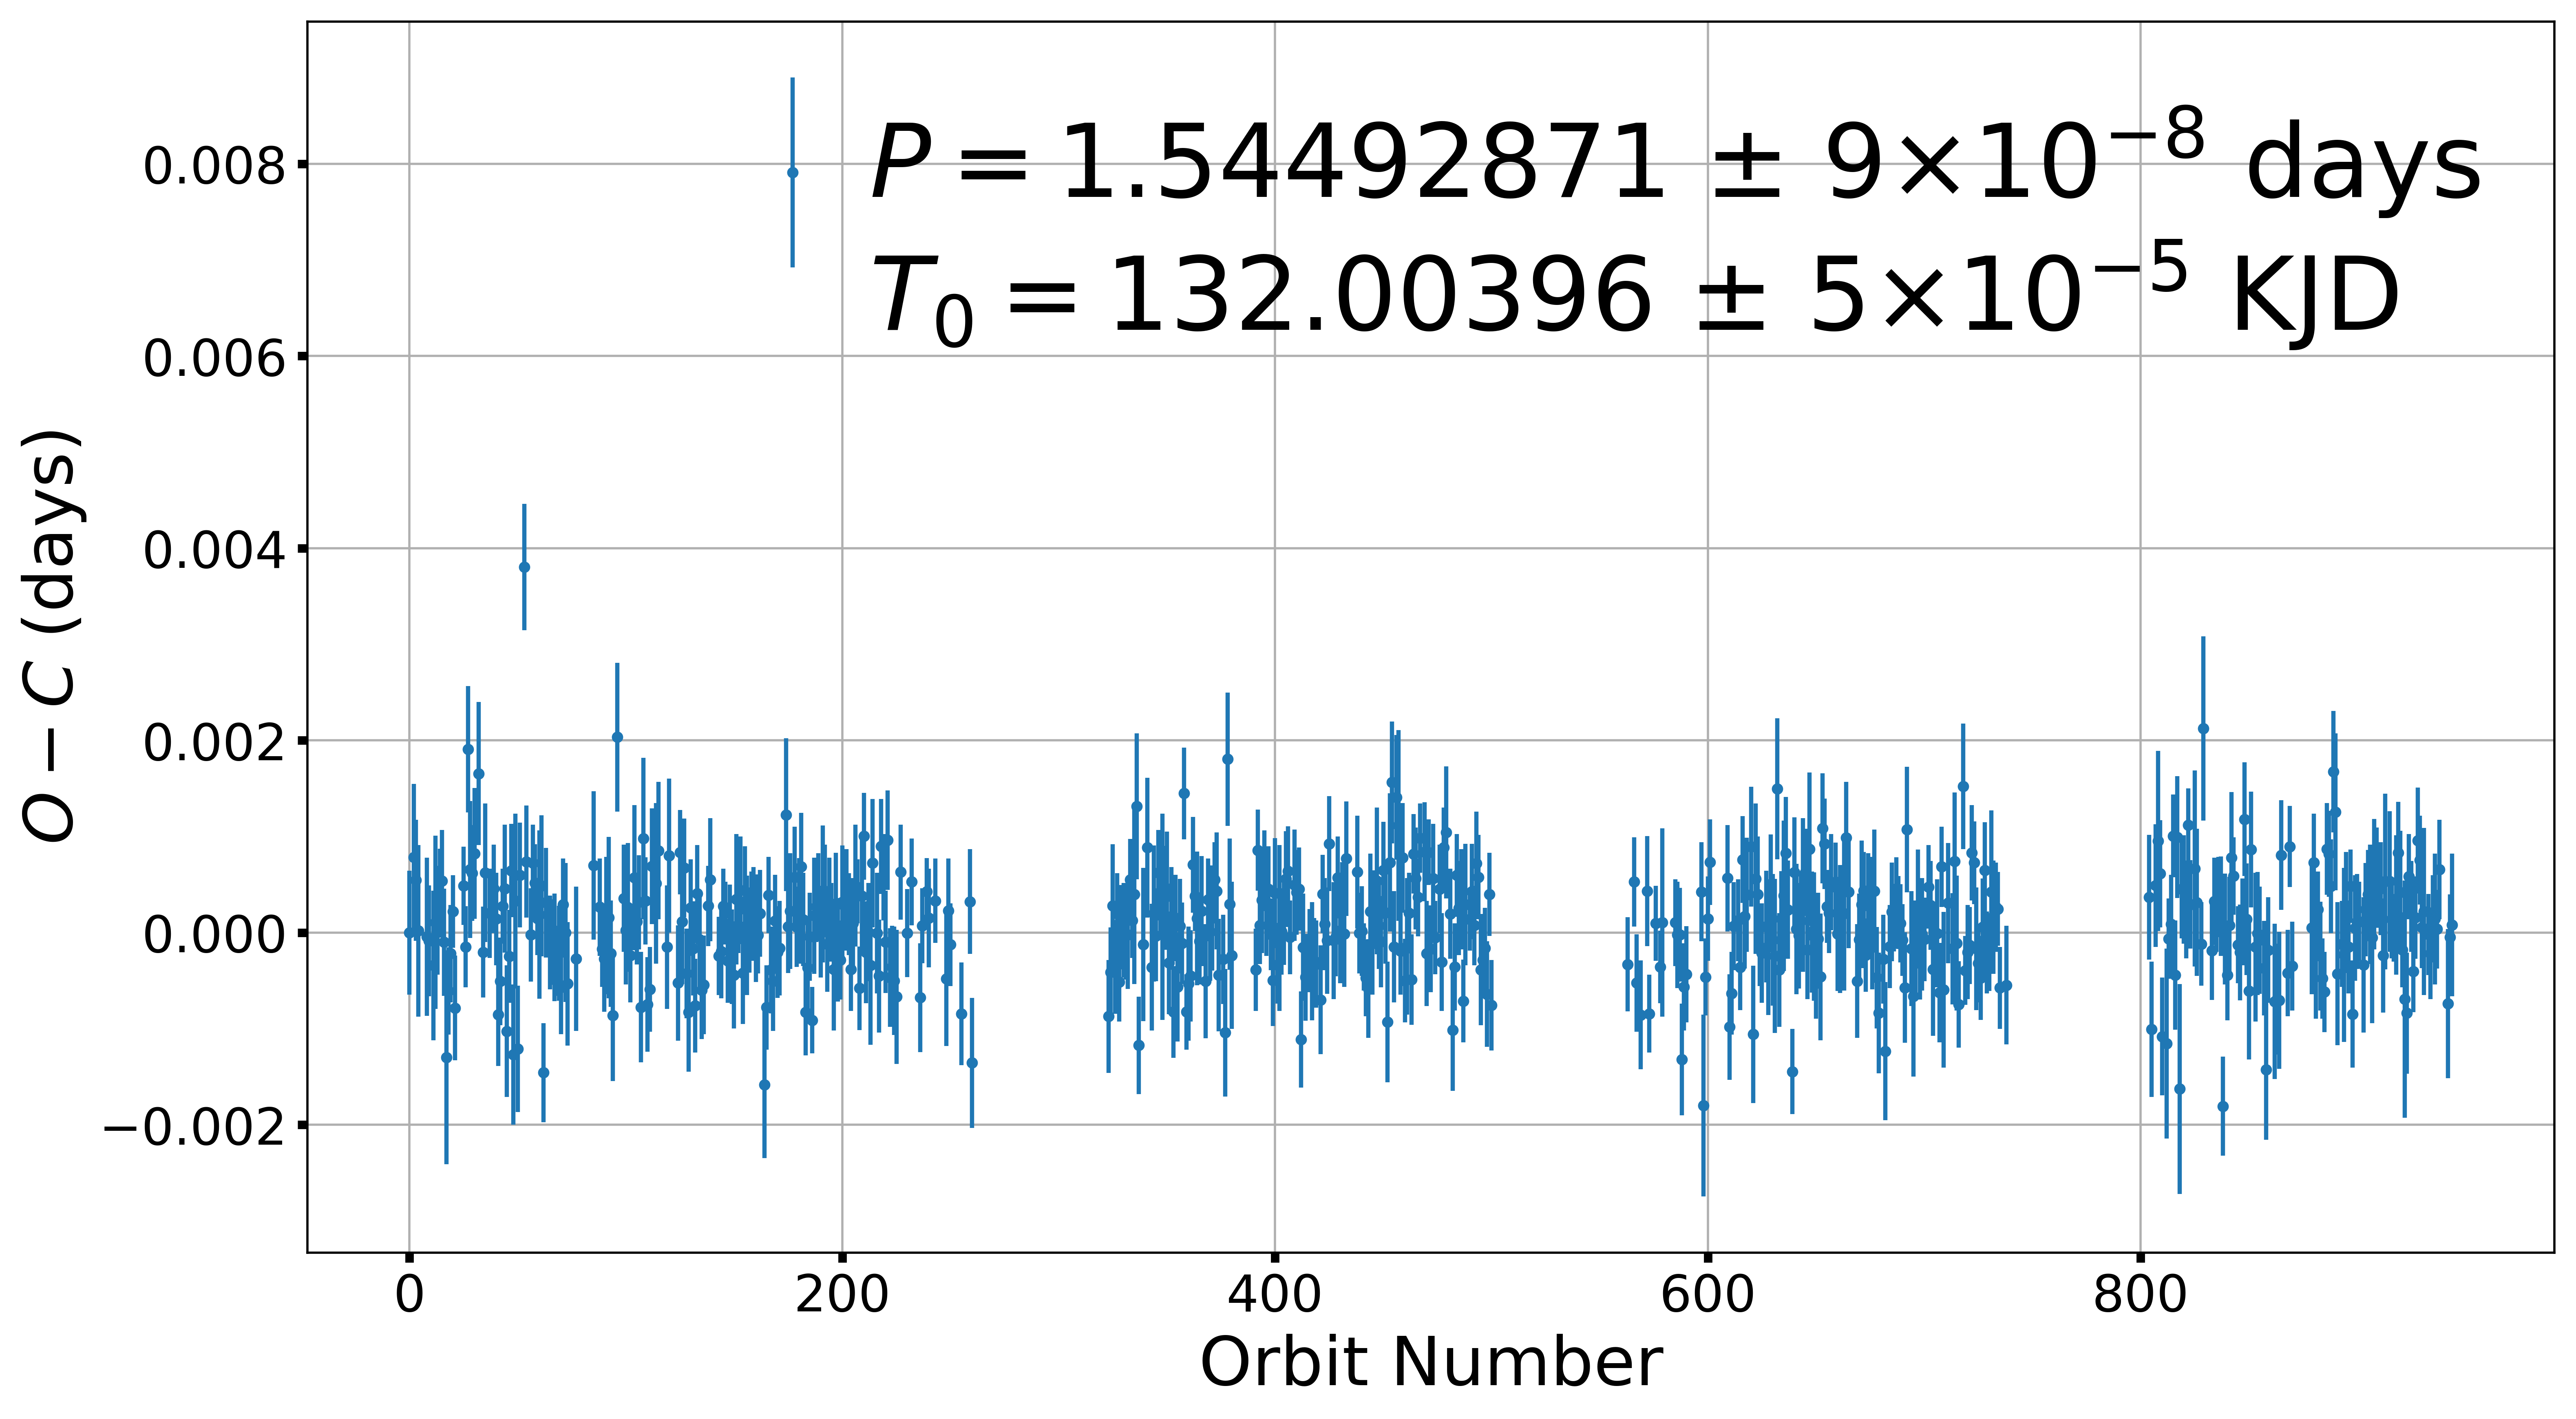
\includegraphics[width=\textwidth]{TTVs_Analysis_of_Kepler76b.png}
    \caption{The observed mid-transit times ($O$) compared to those calculated ($C$) from a linear ephmeris. The period $P$ initial mid-transit time $T_0$ are shown. The gaps in the data near orbit numbers 300, 550, and 800 represent gaps in the available \kepler\ data.\label{fig:TTVs_Analysis_of_Kepler76b}}
\end{figure}

\begin{figure}
    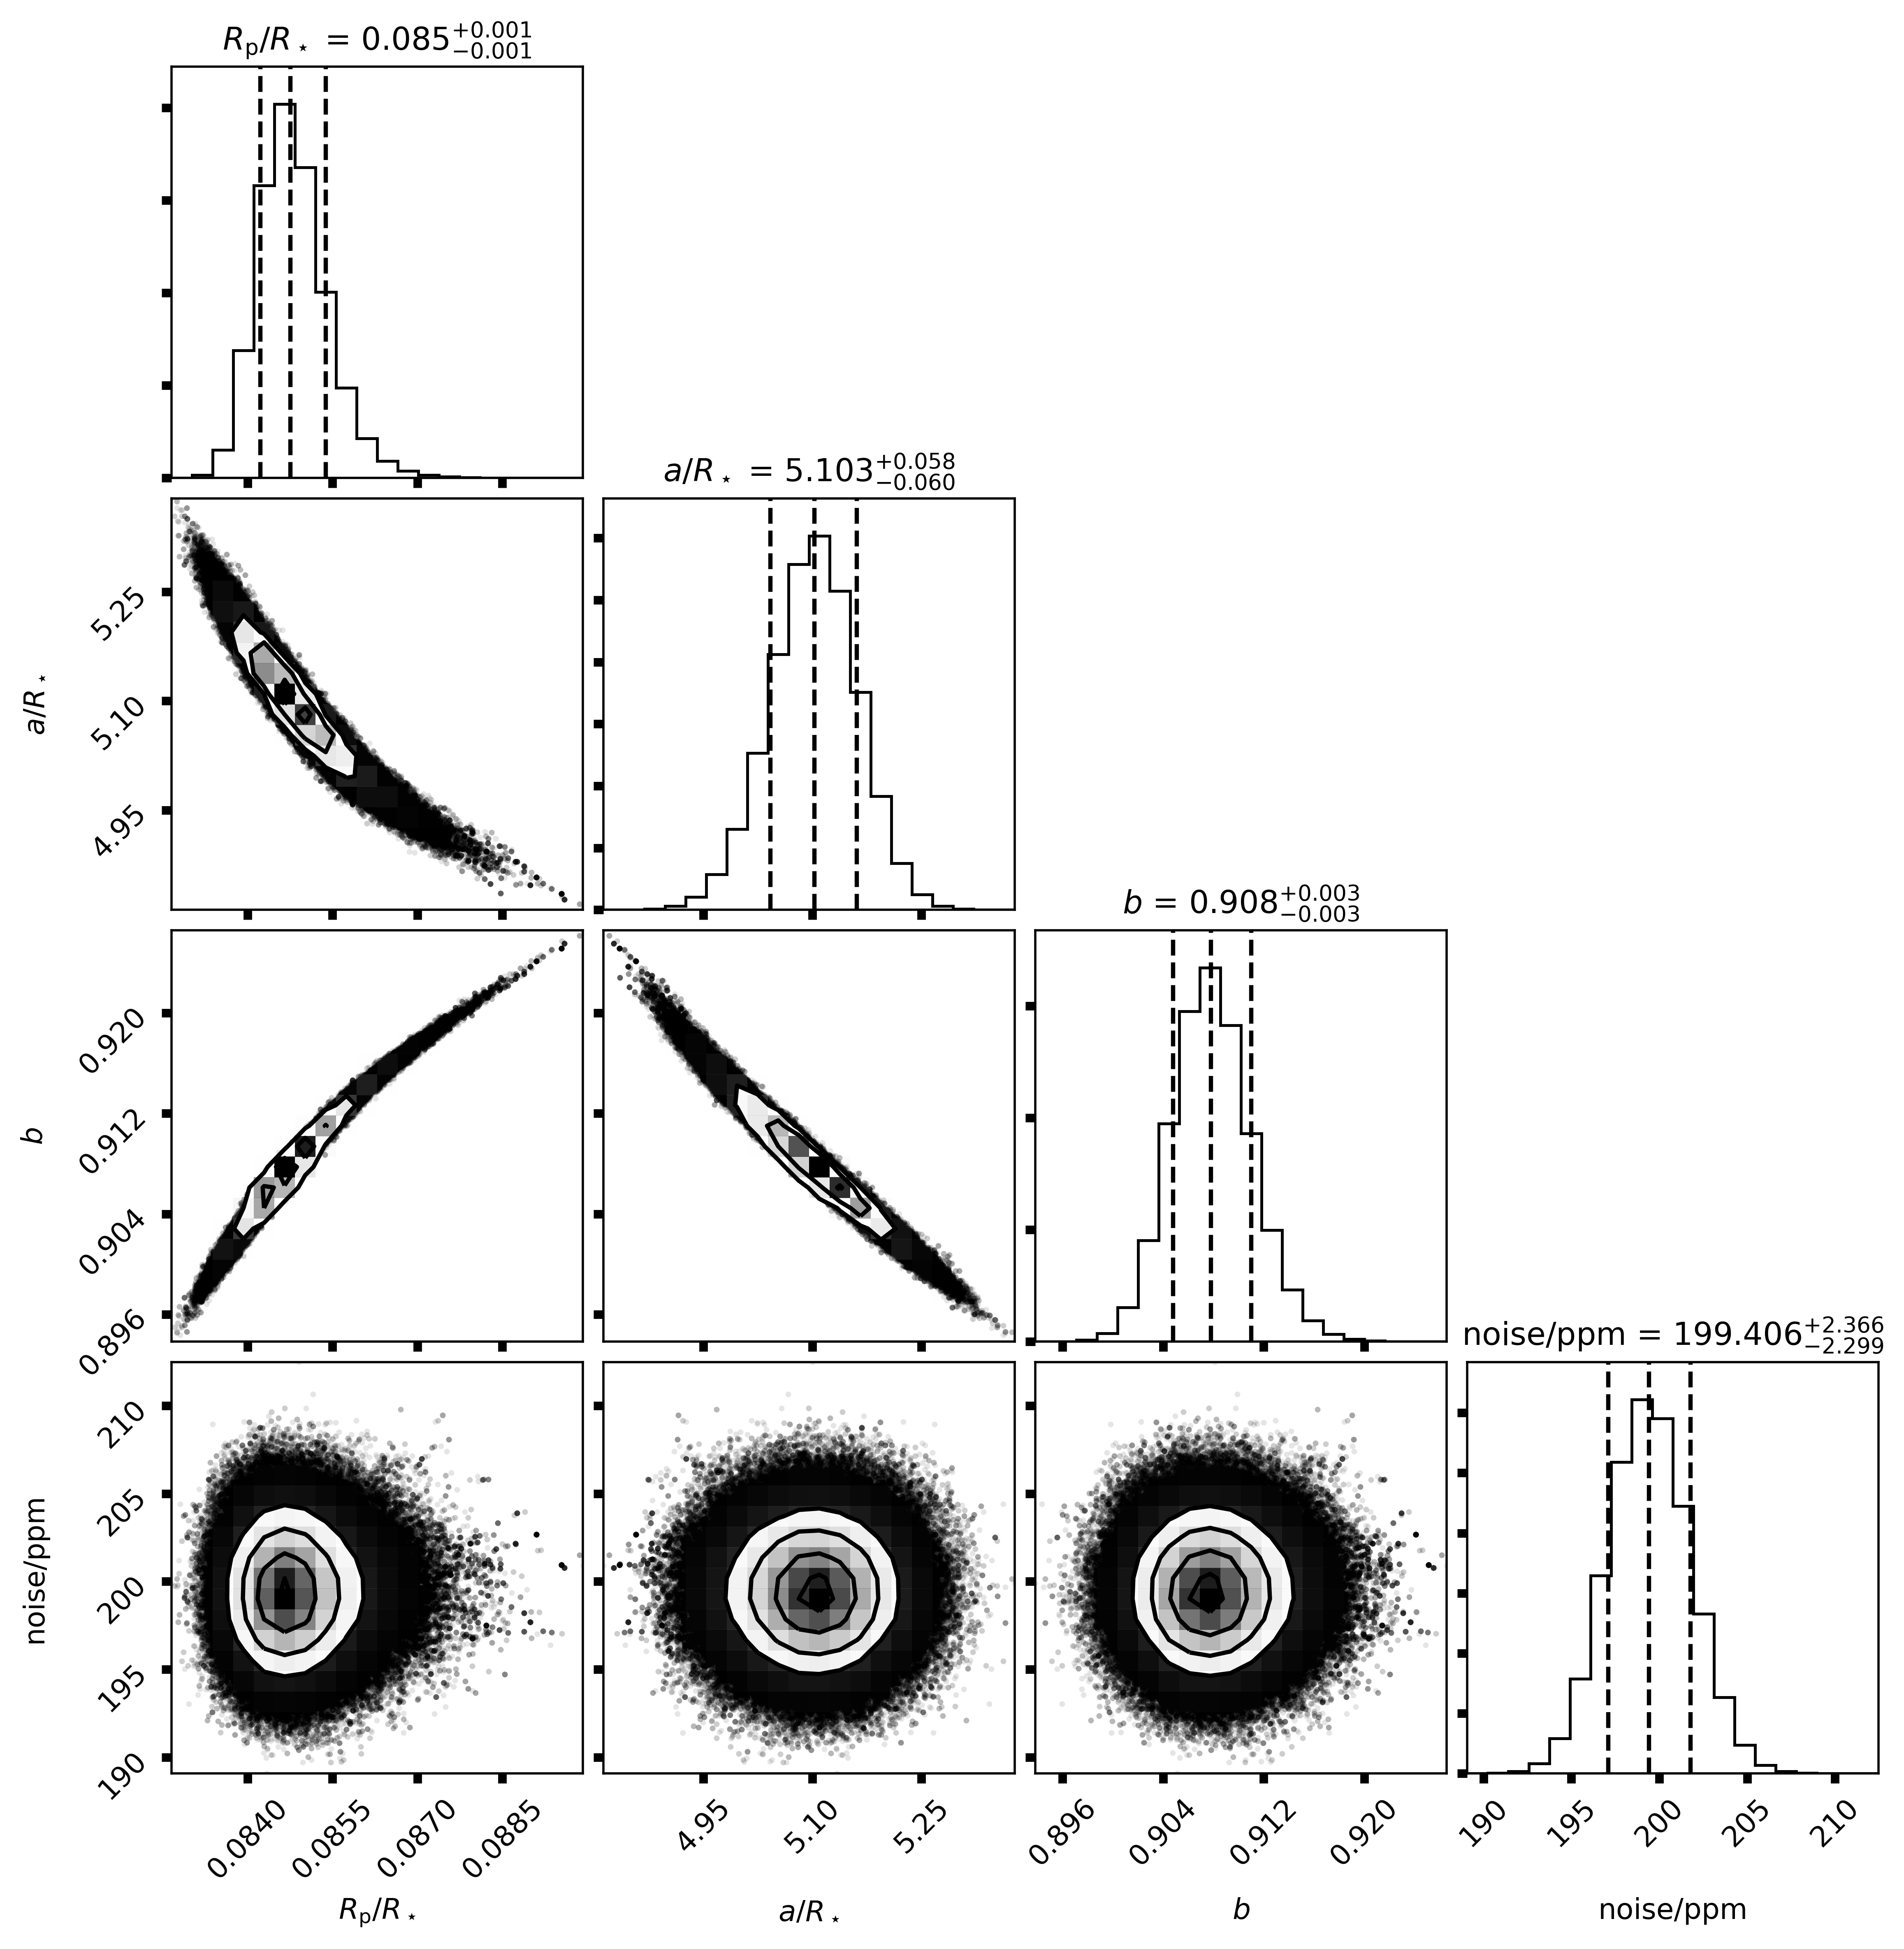
\includegraphics[width=\textwidth]{folded-transit-corner-plot_Analysis-of-Kepler76b.png}
    \caption{The distributions of best-fit parameters for all the data phase-folded on the ephemeris shown in Figure \ref{fig:TTVs_Analysis_of_Kepler76b}: the planet-star radius ratio $R_{\rm p}/R_\star$, the ratio of the planet's orbital semi-major axis to the stellar radius $a/R_\star$, the impact parameter $b$, and an estimate of the per-point noise in parts-per-million (ppm). The histograms along the top-right of each row/column shows the distribution for a parameter marginalized over all the other parameters, while distributions in the shaded contour plots are marginalized over the parameters not labeled to illustrate the correlations between parameters. For example, in the $b$-$R_p/R_\star$ contour plot, the best-fitting $b$-value increases as the $R_p/R_\star$-value increases.}
    \label{fig:folded-transit-corner-plot_Analysis-of-Kepler76b}
\end{figure}

\begin{figure}
    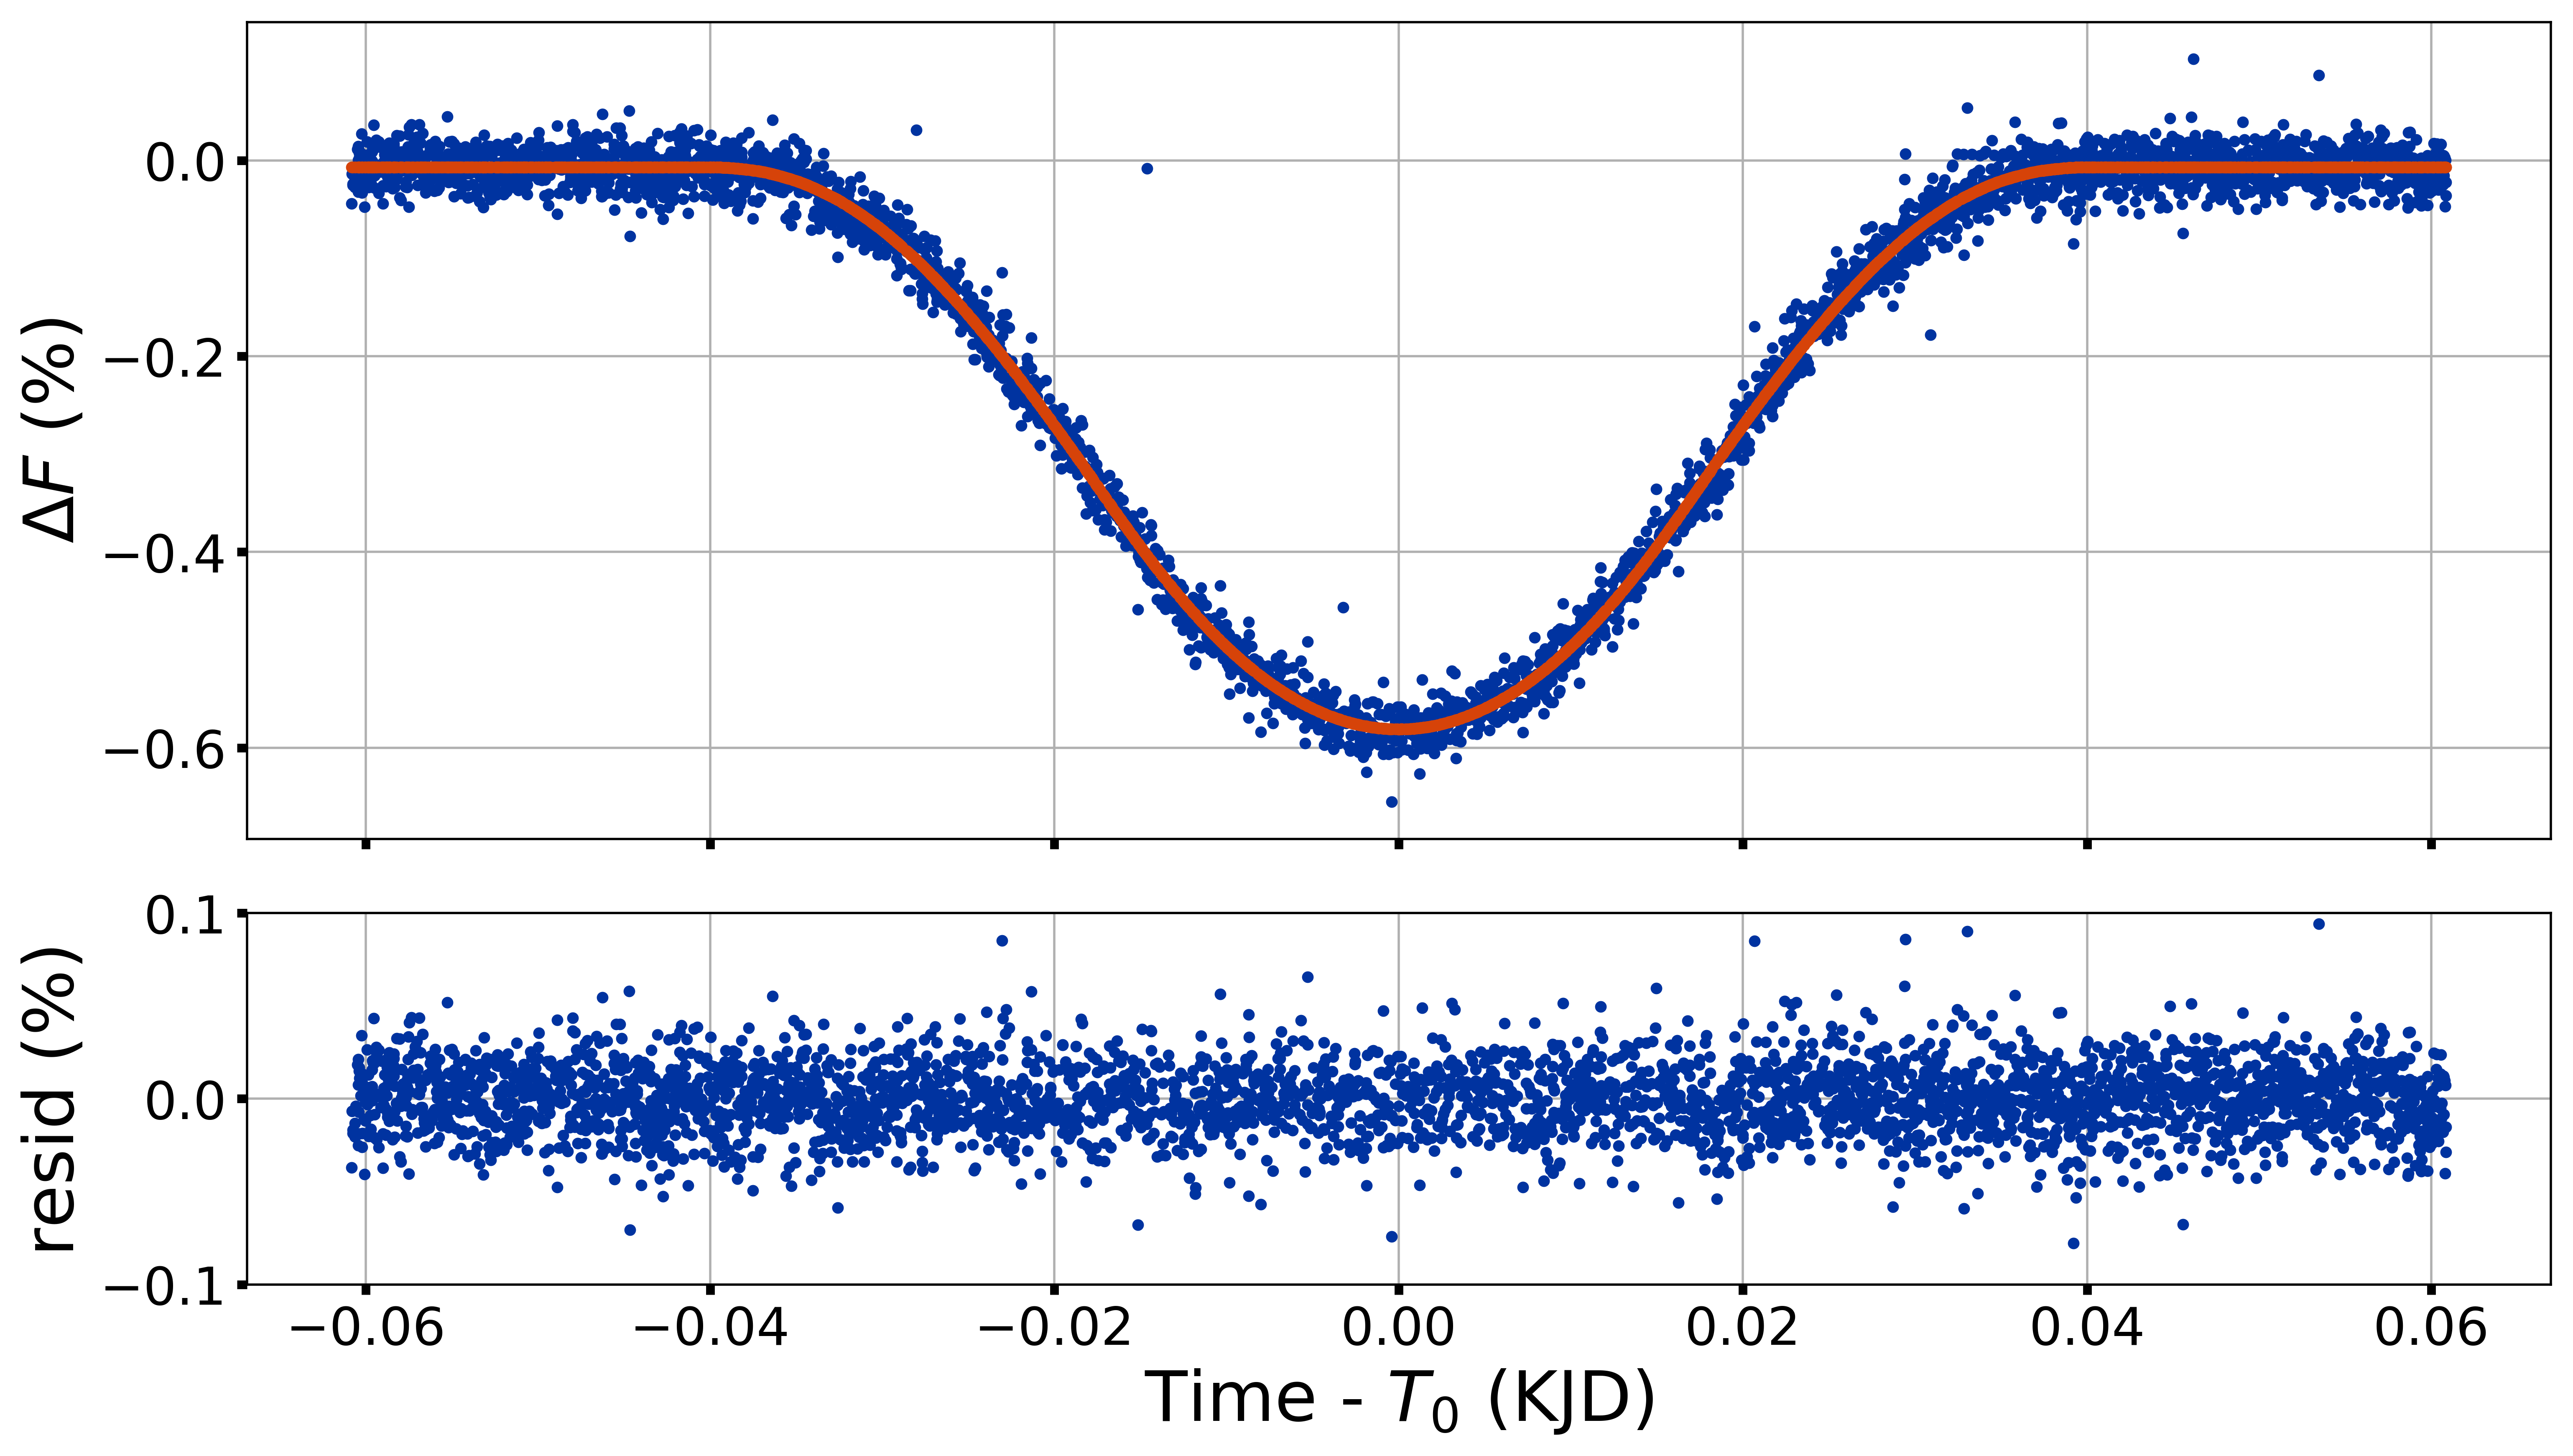
\includegraphics[width=\textwidth]{final_best_fit_transit_Analysis_of_Kepler76b.png}
    \caption{The top panel shows best-fit transit curve for all the in-transit data phase-folded on the ephemeris shown in Figure \ref{fig:TTVs_Analysis_of_Kepler76b}, with residuals between the model (orange line) and data (blue points) in the bottom panel.\label{fig:final_best_fit_transit_Analysis_of_Kepler76b}}
\end{figure}

\begin{figure}
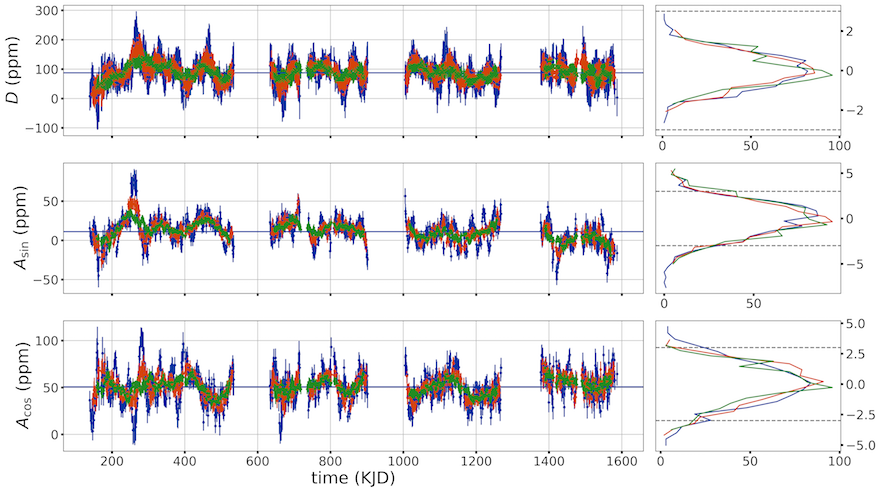
\includegraphics[width=\textwidth]{planet-phase-curve-var_Analysis_of_Kepler76b.png}
\caption{The leftmost three panels show variations over time in the eclipse depth $D$ and amplitudes $A_{\rm sin}$ and $A_{\rm cos}$ after stacking and folding data points from consecutive orbits in a window 10 orbits wide (blue points), 20 orbits wide (orange points), and 40 orbits wide (green points). The blue horizontal lines show the best-fit average values for each parameter. The rightmost panels show histograms of how much $D$, $A_{\rm sin}$, and $A_{\rm cos}$ deviate from their respective average values, normalized to their respective uncertainties, and the dashed grey lines illustrate $\pm$3-$\sigma$. \label{fig:planet-phase-curve-var_Analysis_of_Kepler76b}}
\end{figure}

\begin{figure}
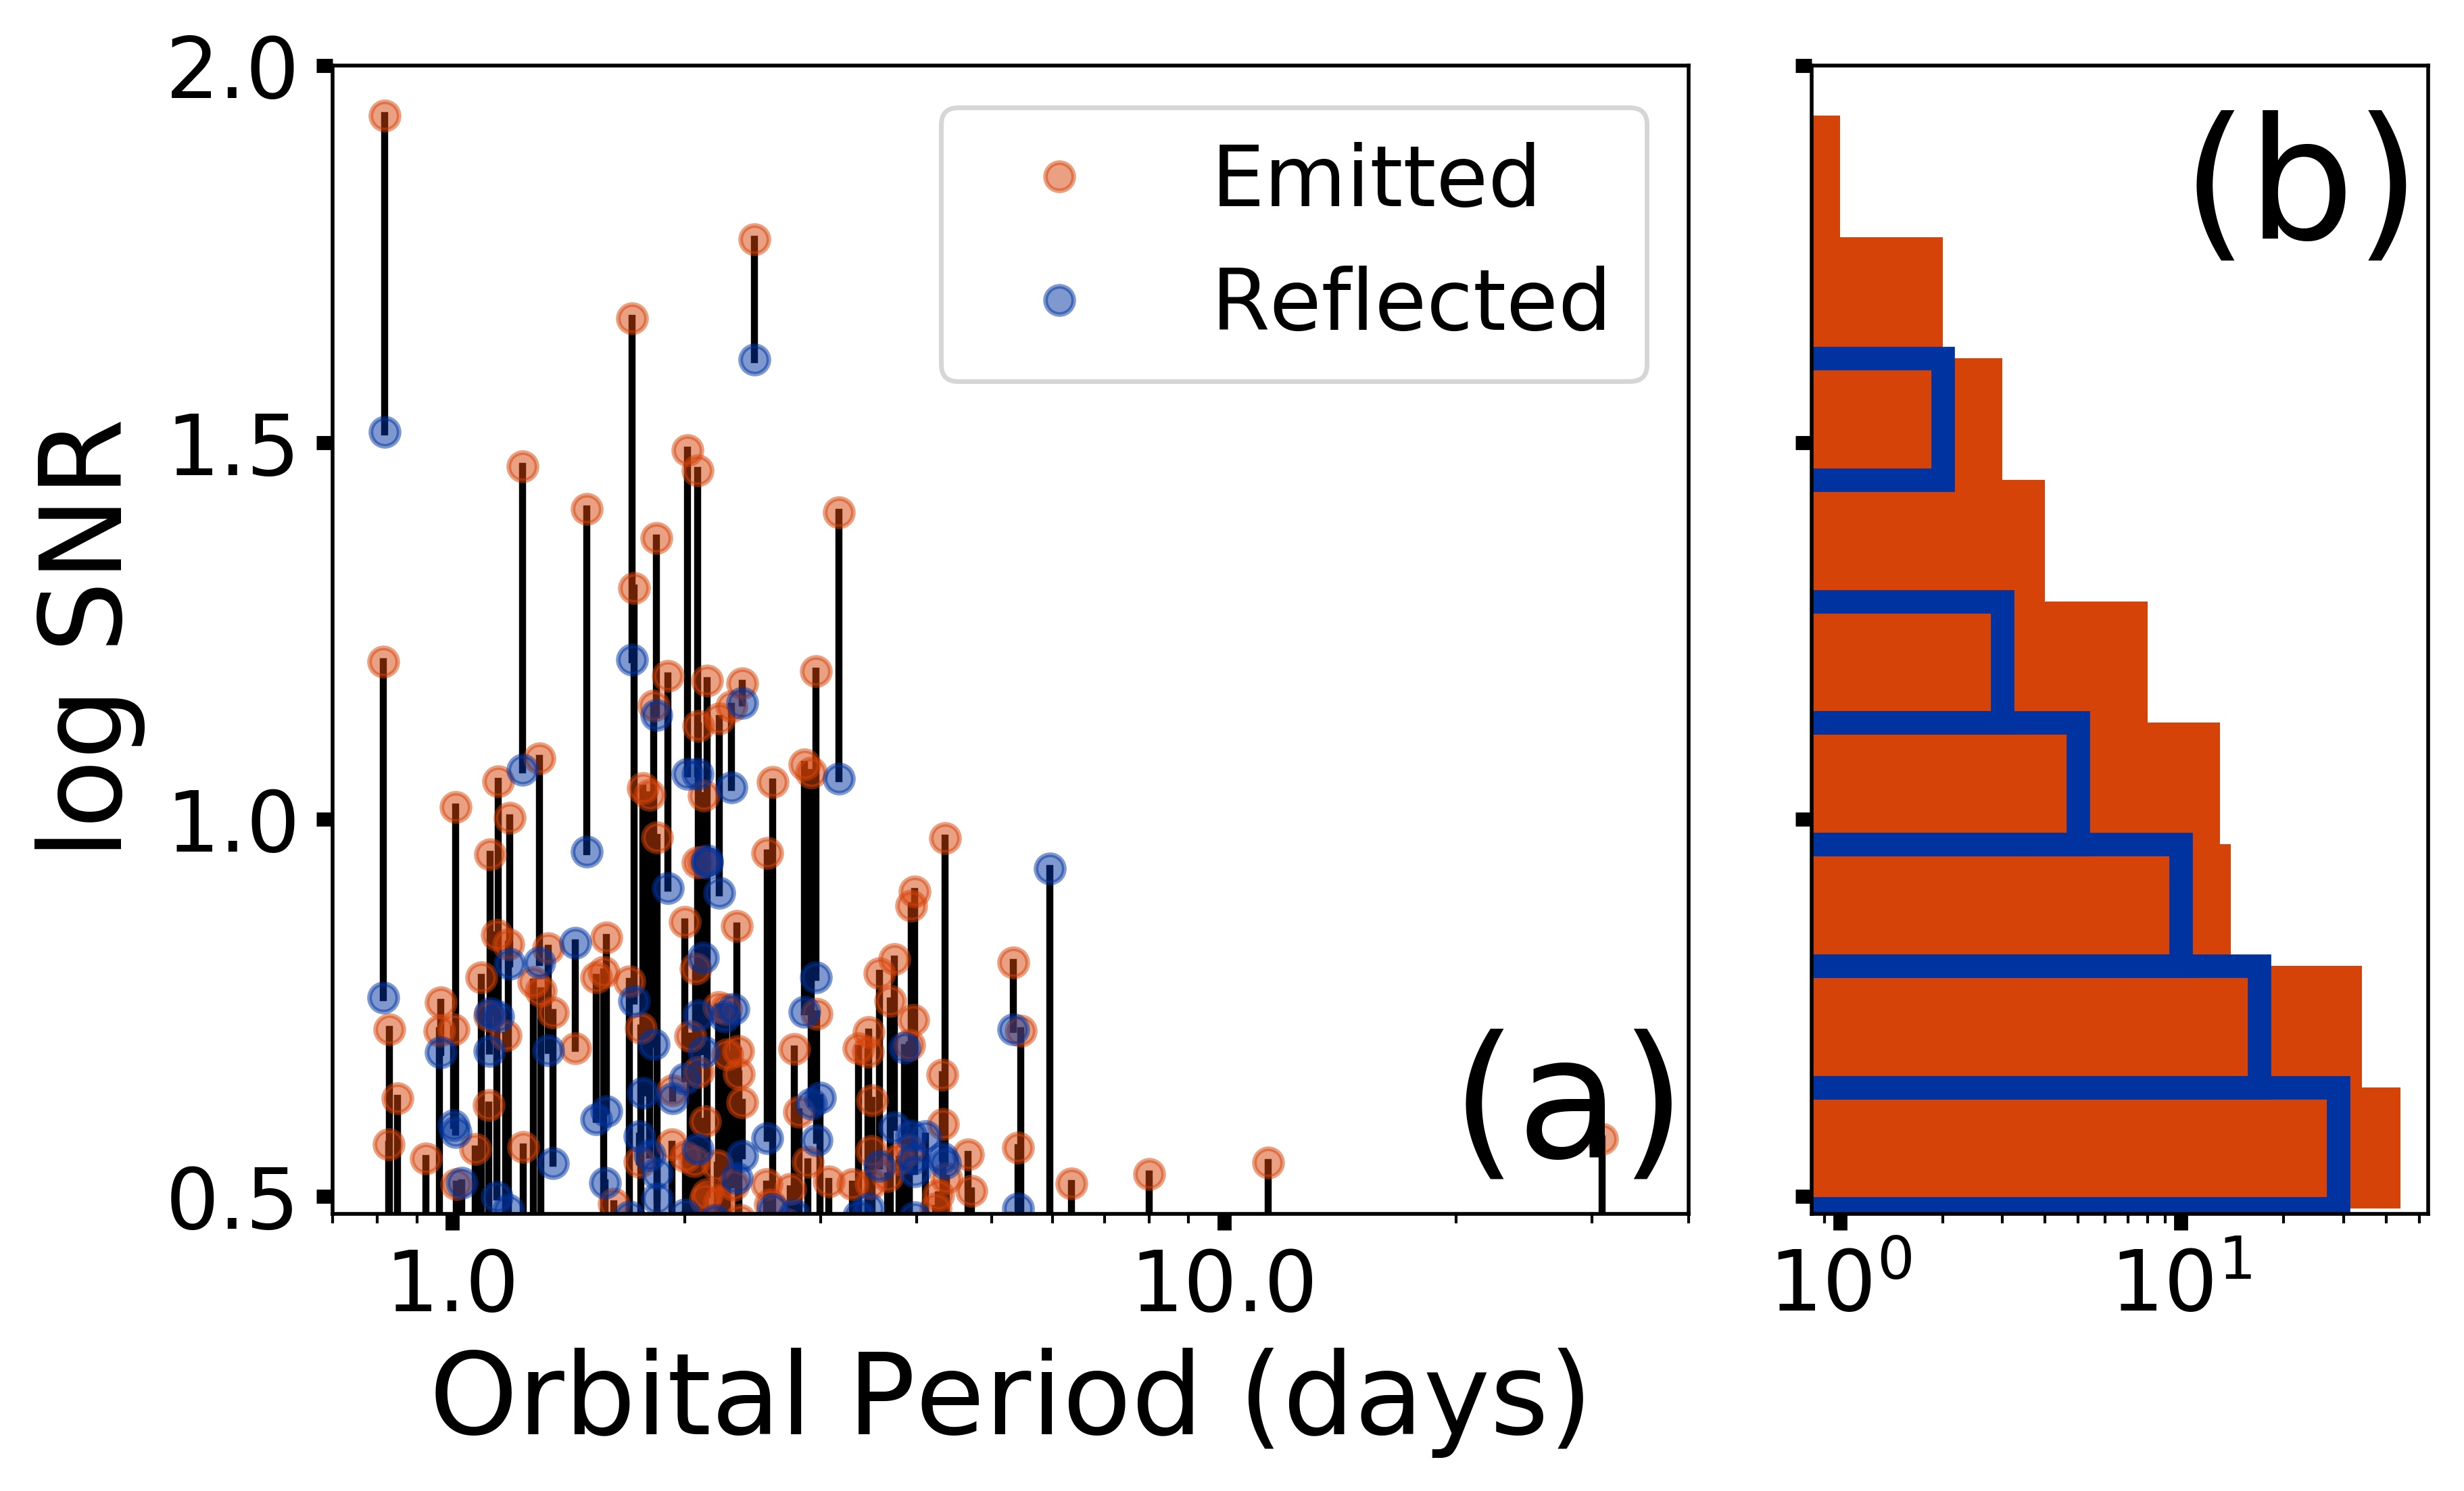
\includegraphics[width=\textwidth]{eclipse_estimates.jpg}
\caption{The $\log$ of the signal-to-noise ratio $SNR$ for planetary secondary eclipses for a population of synthetic planets from the \tess\ mission yield study of \citet{2018arXiv180405050B}. The blue dots in (a) show eclipses for perfectly reflecting planets, while the orange dots show eclipses for perfect blackbody planets, with black lines connecting the two eclipses for each planet. Panel (b) shows a histogram of SNR-values. \label{fig:eclipse_estimates}}
\end{figure}

\end{document}